\documentclass{beamer}
\definecolor{links}{HTML}{2A1B81}
\hypersetup{colorlinks,linkcolor=,urlcolor=blue}
\usepackage[utf8]{inputenc}
\usepackage{graphicx}
\usepackage{booktabs}
\usepackage{ragged2e}
\usepackage{xcolor}
\definecolor{LightGray}{gray}{0.975}

\usepackage{tikz}
\usetikzlibrary{arrows,shapes}

\usepackage{algorithm}
\usepackage{algorithmic}

\usepackage{minted}
\usepackage{xcolor}
\definecolor{LightGray}{gray}{0.975}

\usepackage{listings}

%\usetheme{Warsaw}
\usefonttheme{serif} 

\title[Metadata]{Database Administration}
\subtitle{Lecture 03: What is Metadata?}
\author{Coronel, Morris \& Post}
\date{\today}

\setbeamertemplate{navigation symbols}{}%remove navigation symbols

\defbeamertemplate*{footline}{shadow theme}
{%
  \leavevmode%
  \hbox{\begin{beamercolorbox}[wd=.5\paperwidth,ht=2.5ex,dp=1.125ex,leftskip=.3cm plus1fil,rightskip=.3cm]{author in head/foot}%
    \usebeamerfont{author in head/foot} Database Administration \hfill \insertshorttitle
  \end{beamercolorbox}%
  \begin{beamercolorbox}[wd=.5\paperwidth,ht=2.5ex,dp=1.125ex,leftskip=.3cm,rightskip=.3cm plus1fil]{title in head/foot}%
    \usebeamerfont{title in head/foot} \hfill \insertframenumber\,/\,\inserttotalframenumber%
  \end{beamercolorbox}}%
  \vskip0pt%
}

\AtBeginSection[]
{
     \begin{frame}<beamer>
     \frametitle{Plan}
     \tableofcontents[currentsection]
     \end{frame}
}

\newcommand{\toRight}[1]{
    \begin{FlushRight}
        {\tiny #1}
    \end{FlushRight}
} % Align to right

\begin{document}

\frame{\titlepage}

\begin{frame}{Database Administration: What is Metadata?.}
    \centering
    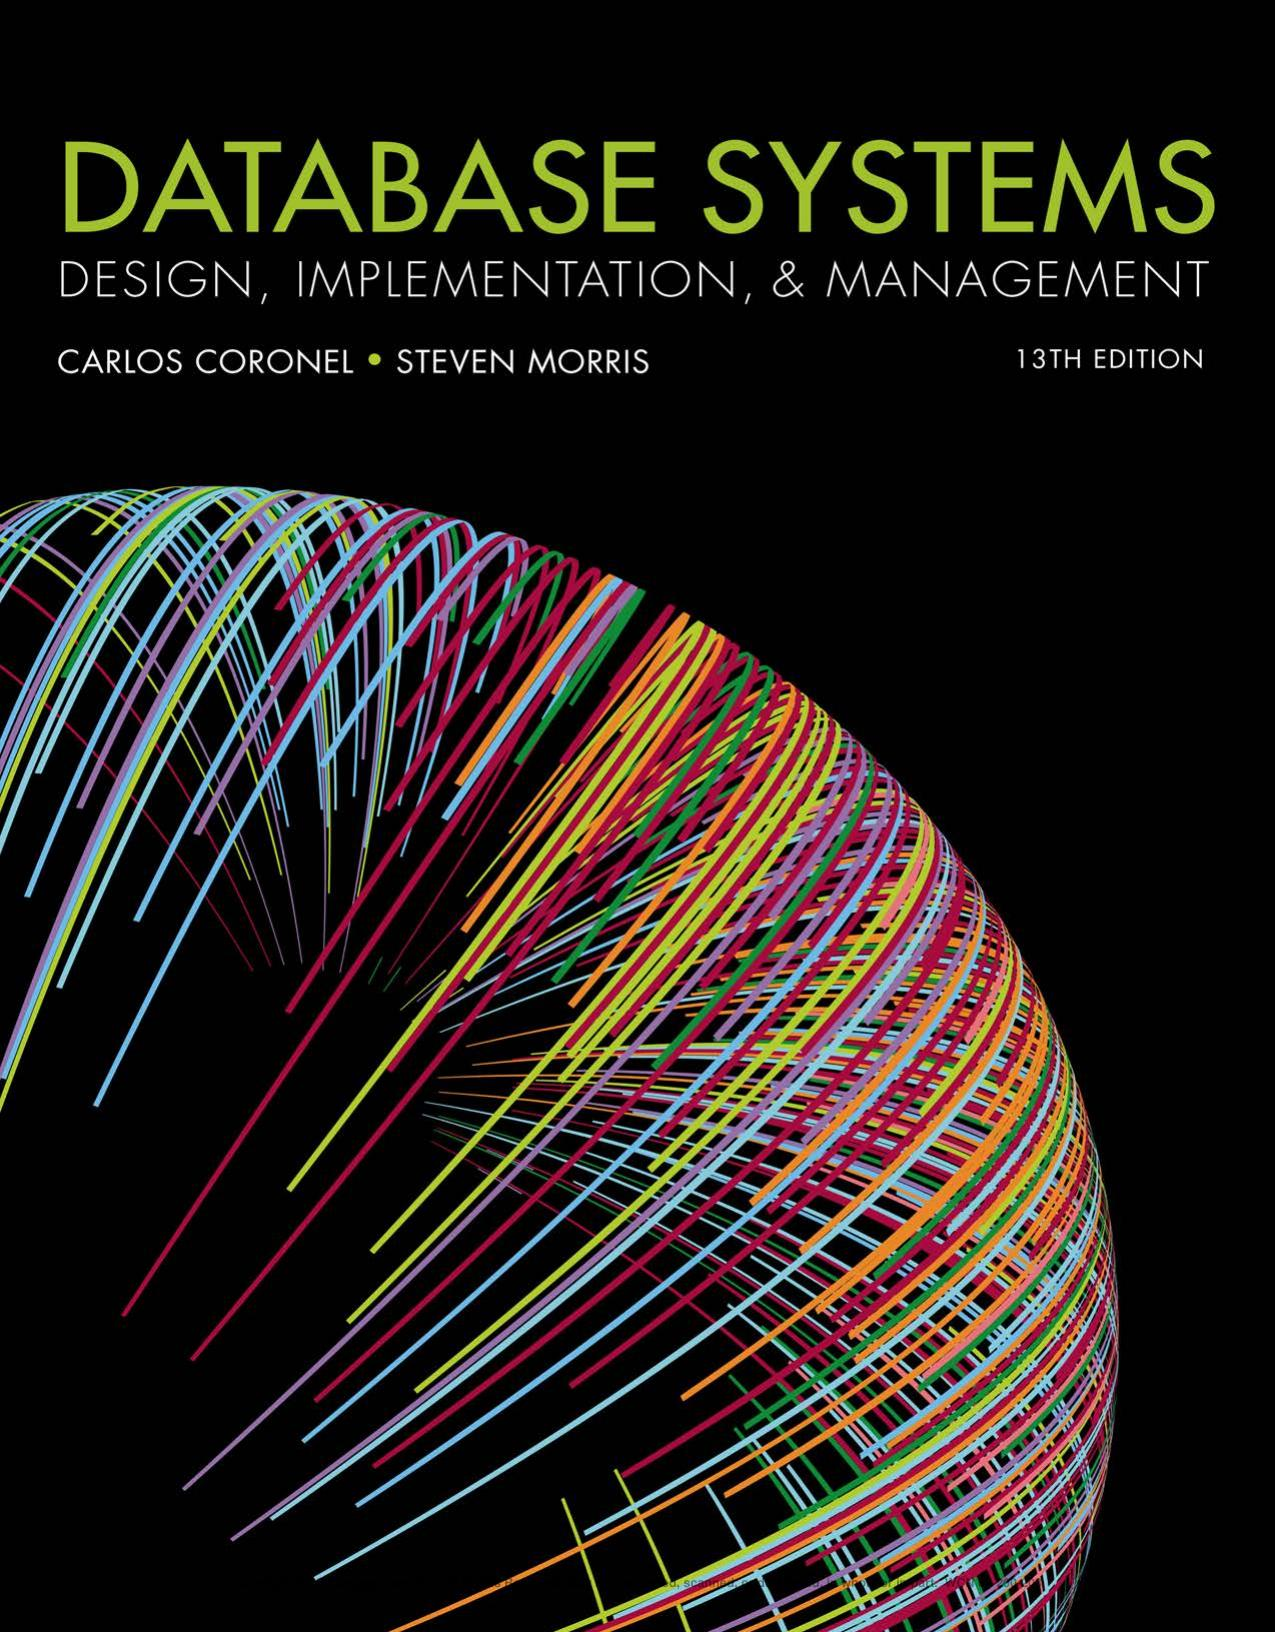
\includegraphics[width=0.34\textwidth]{figures/book_cover2.jpg}
    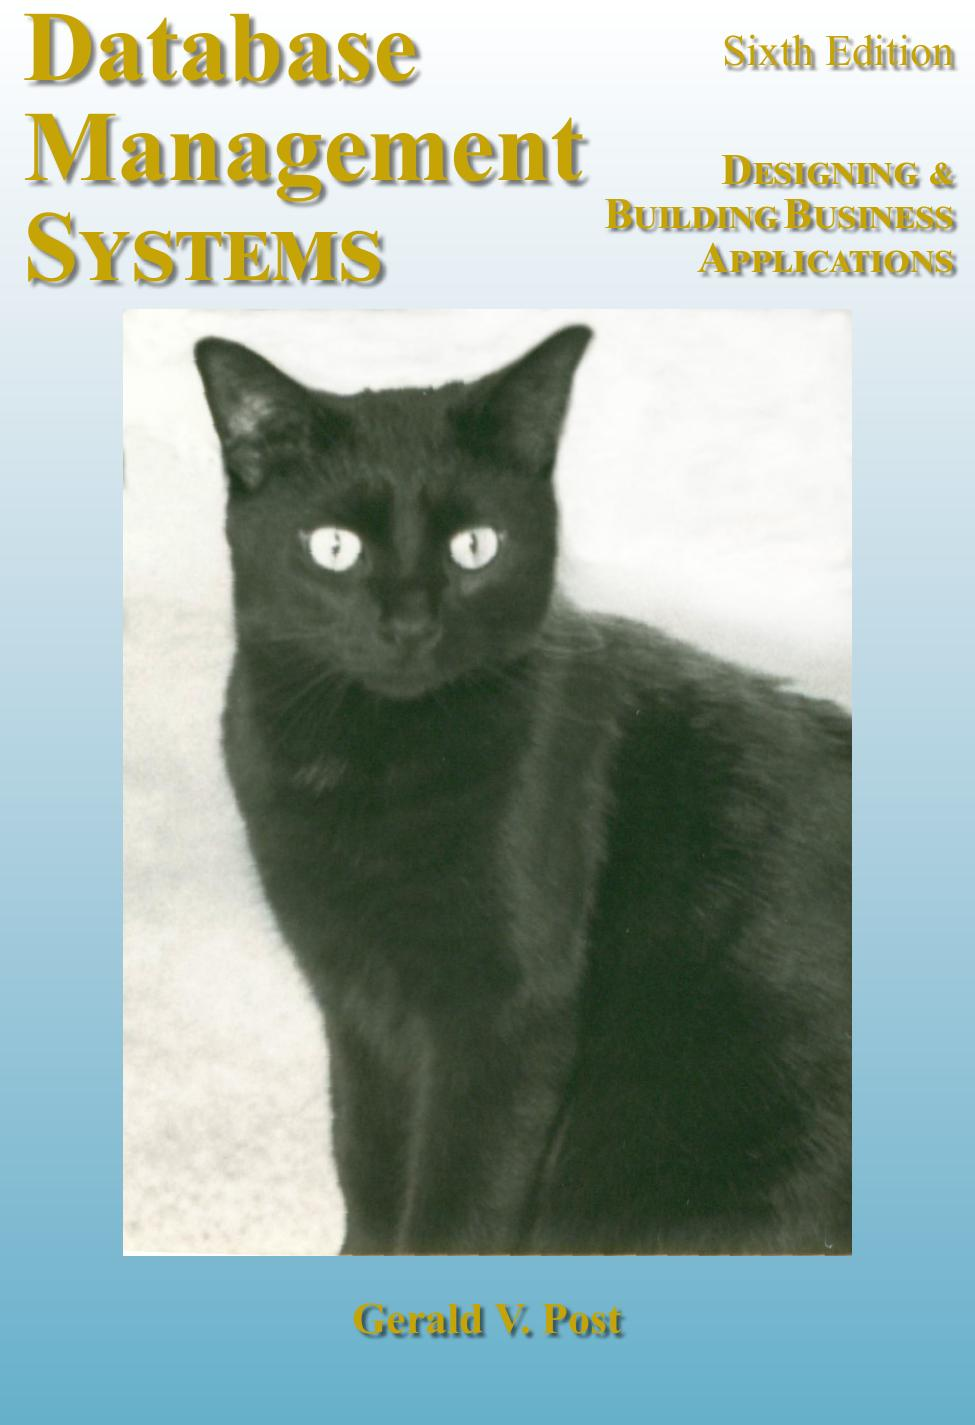
\includegraphics[width=0.3\textwidth]{figures/book_cover3.jpg} \\
    \vspace{5mm}
    {
        \tiny
        Content has been extracted from \textit{Database Systems: Design, Implementation, and Management.}, 13th Edition, by Carlos Coronel \& Steven Morris. Cengage Learning. 2018. and \textit{Database Management Systems: Designing \& Building Business Applications.}, 6th Edition, by Gerald Post. McGraw-Hill/Irwin. 2014. \\
        Visit \url{https://www.cengage.com/c/database-systems-design-implementation-management-13e-coronel/9781337627900PF/} and \url{https://www.jerrypost.com/database/DBBookSummary.html}.\\
    }
\end{frame}

\section{What is Metadata?}

\begin{frame}{Metadata}
    \begin{itemize}
        \item Metadata is data about data.  Data describing the properties or characteristics of the data: data types, size, domain, range, valid values, ...
    \end{itemize}
    \centering
    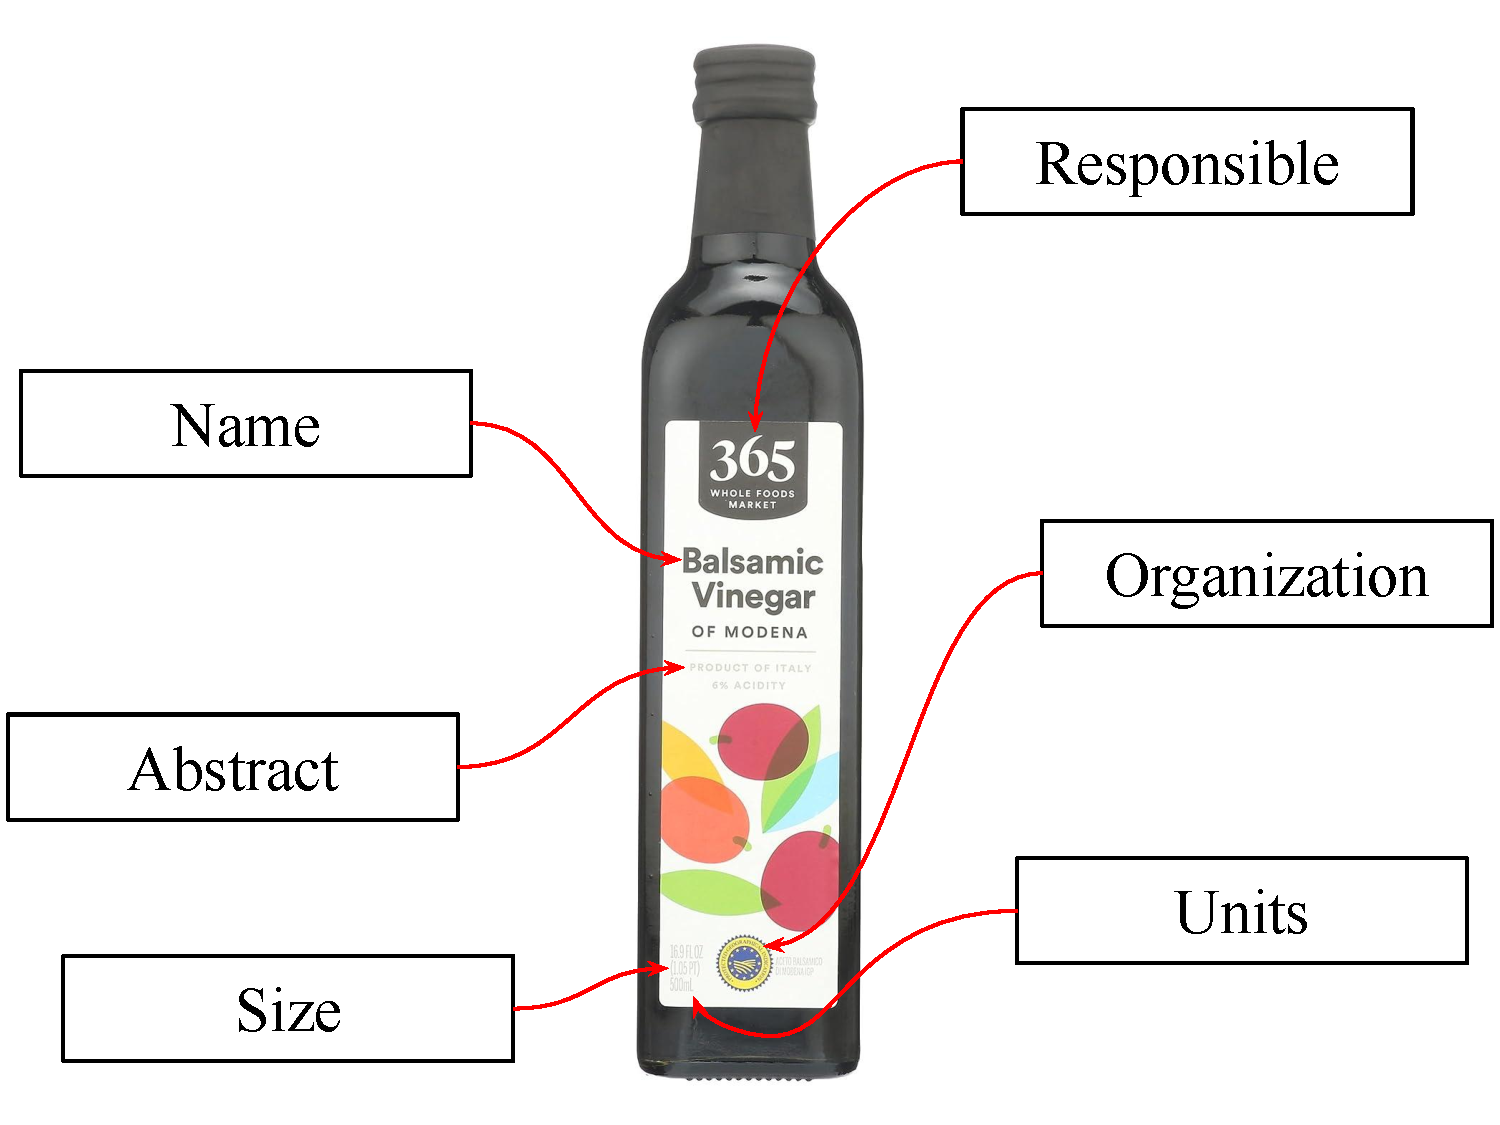
\includegraphics[width=0.75\textwidth]{figures/metadata1}
\end{frame}

\begin{frame}{Metadata}
    \begin{itemize}
        \item Metadata is data about data.  Data describing the properties or characteristics of the data: data types, size, domain, range, valid values, ...
    \end{itemize}
    \centering
    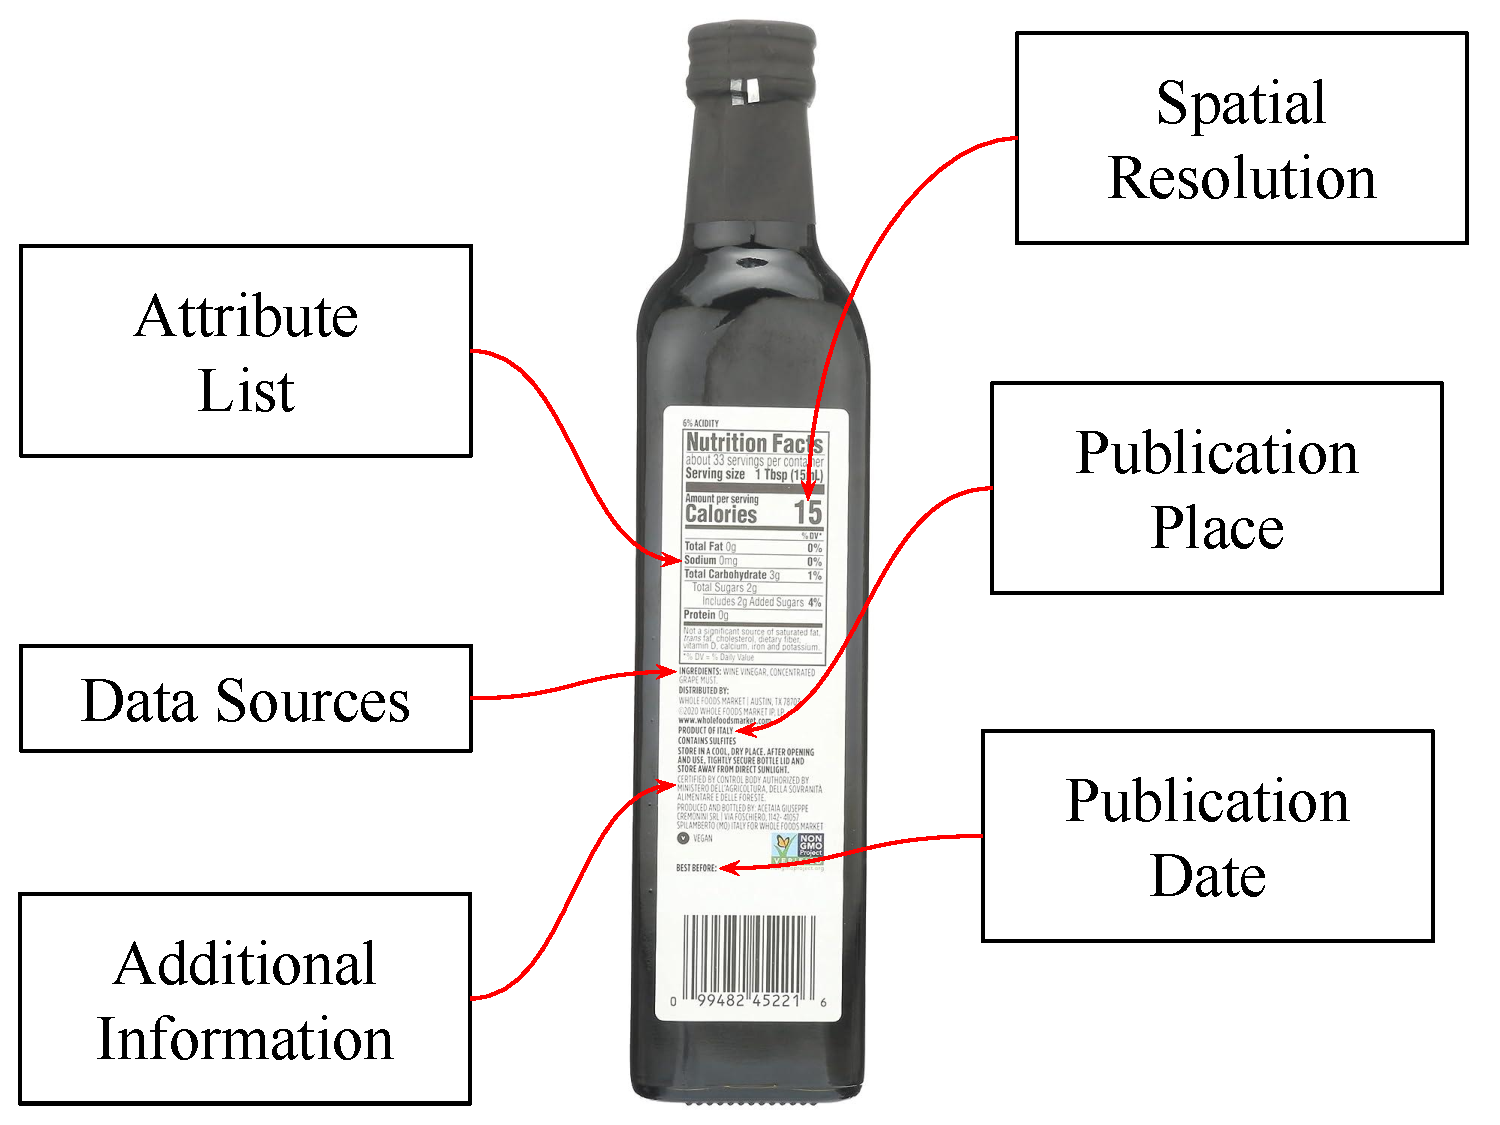
\includegraphics[width=0.75\textwidth]{figures/metadata2}
\end{frame}

\begin{frame}{Metadata}
    \begin{itemize}
        \item Metadata is data about data.  Data describing the properties or characteristics of the data: data types, size, domain, range, valid values, ...
    \end{itemize}
    \centering
    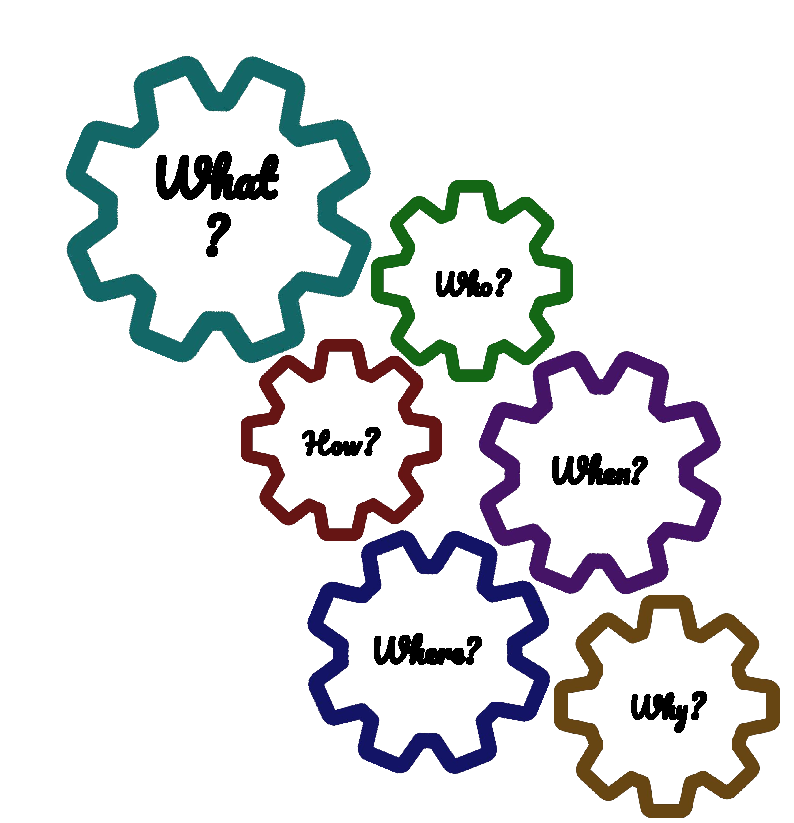
\includegraphics[width=0.55\textwidth]{figures/metadata3}
\end{frame}

\section{Metadata Examples}

\begin{frame}{Photos}
    \centering
    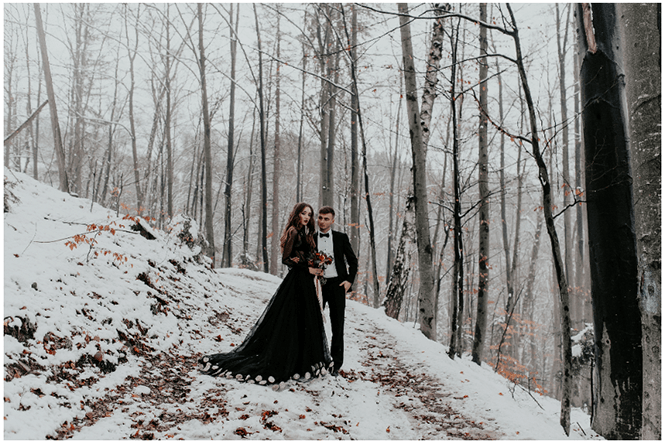
\includegraphics[width=0.75\textwidth]{figures/photo}
\end{frame}
\begin{frame}{Photo Metadata}
    \centering
    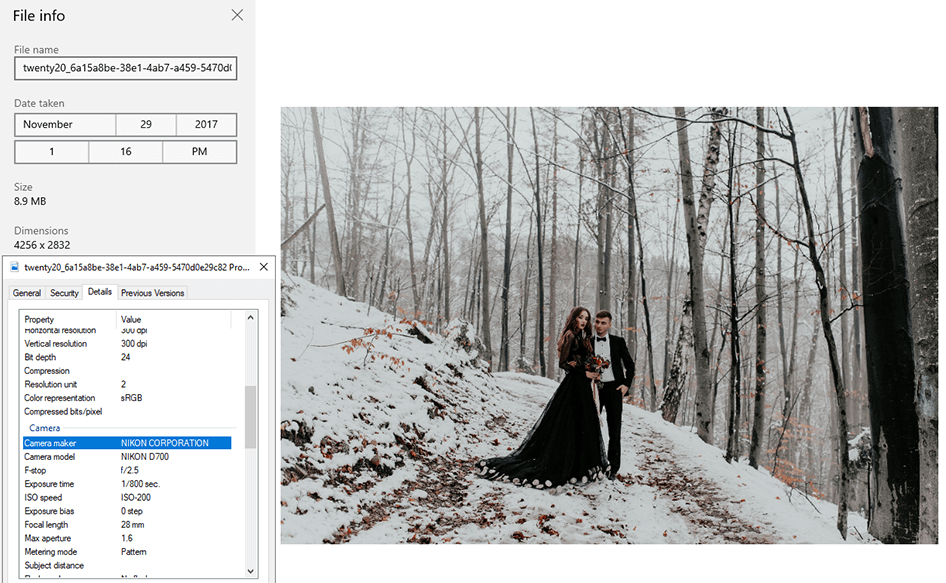
\includegraphics[width=\textwidth]{figures/photometa}
\end{frame}
\begin{frame}{Books}
    \centering
    \fbox{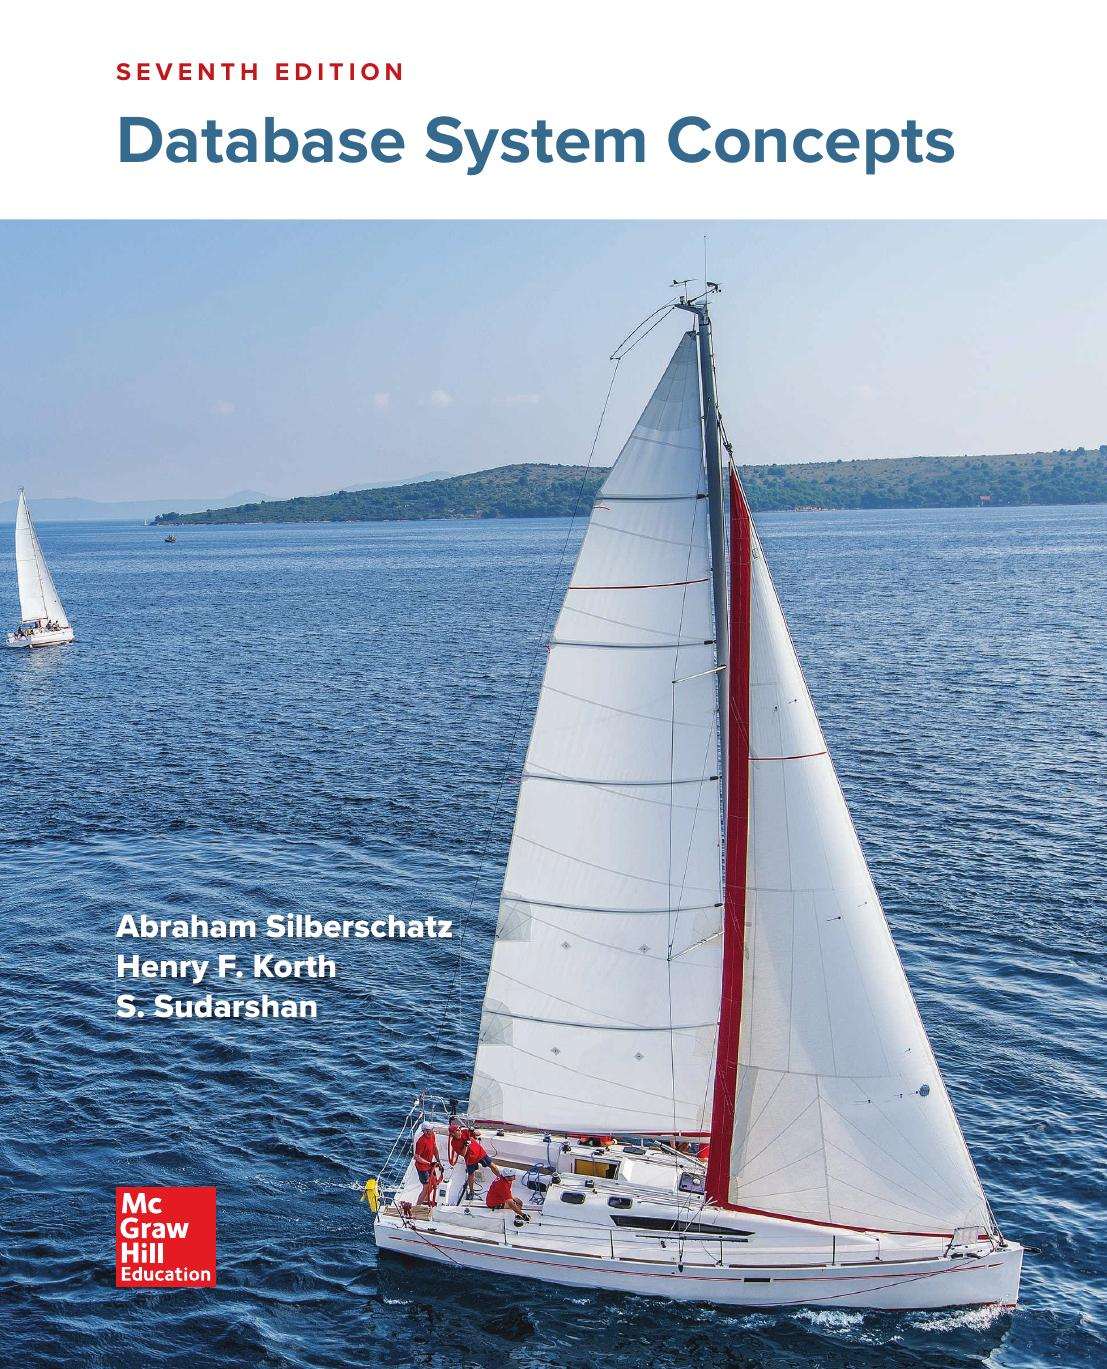
\includegraphics[width=0.45\textwidth]{figures/book}}
\end{frame}
\begin{frame}{Book Metadata}
    \centering
    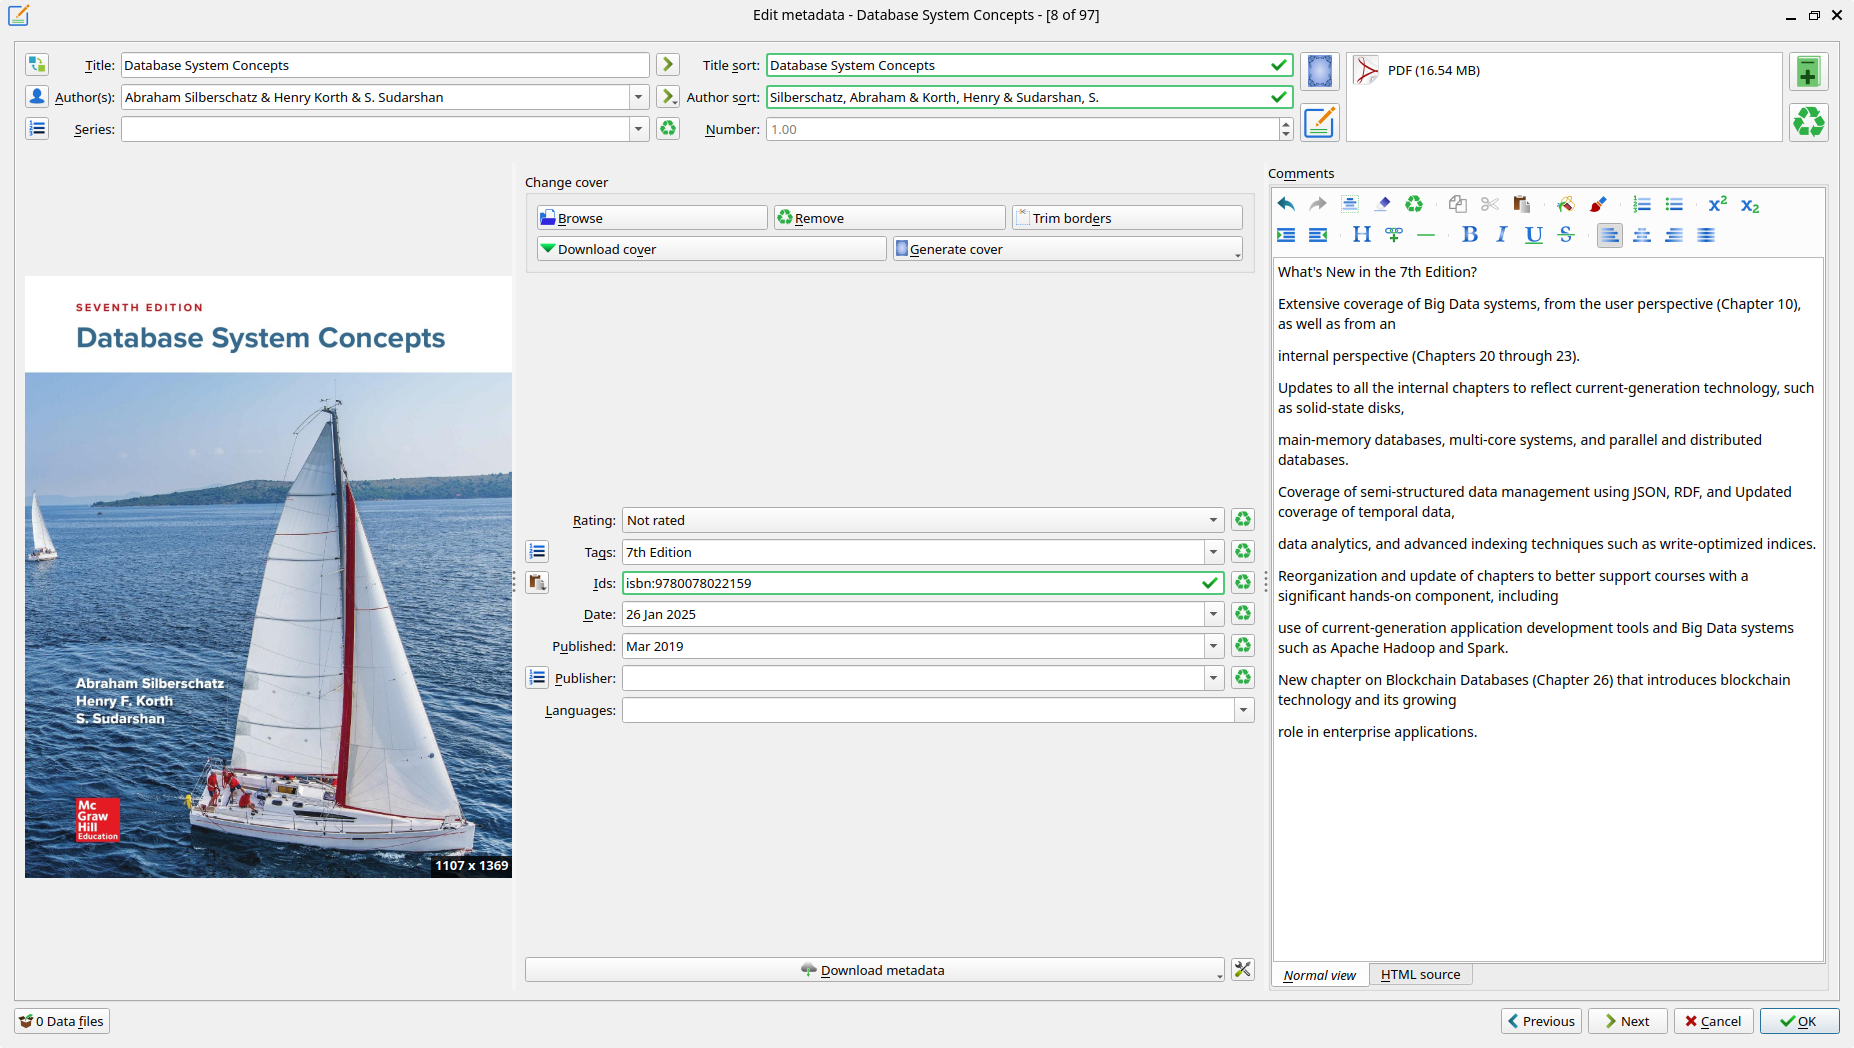
\includegraphics[width=\textwidth]{figures/bookmeta}
\end{frame}
\begin{frame}{Blogs}
    \centering
    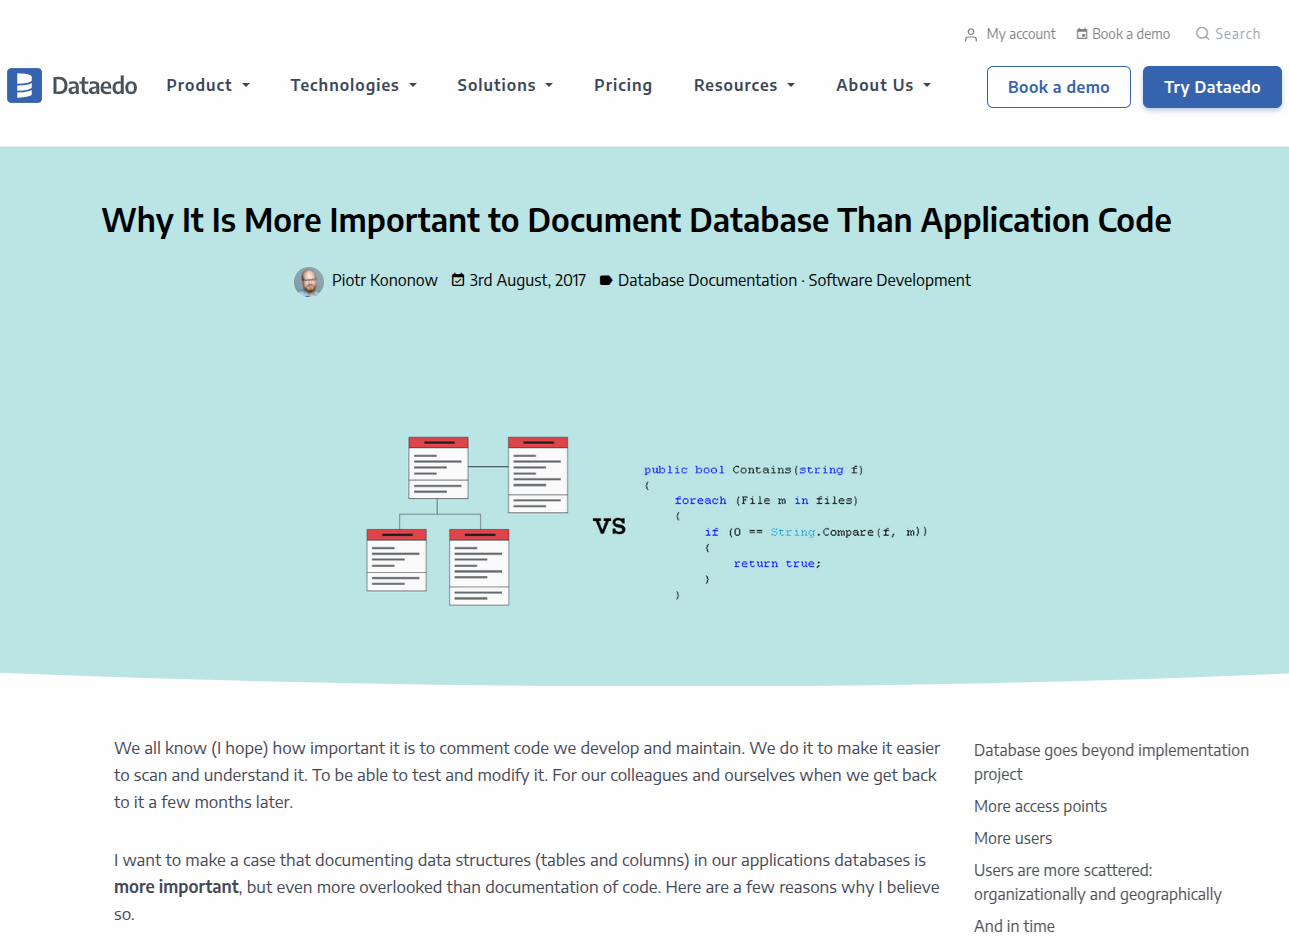
\includegraphics[width=\textwidth]{figures/blog}
\end{frame}
\begin{frame}{Blog Metadata}
    \centering
    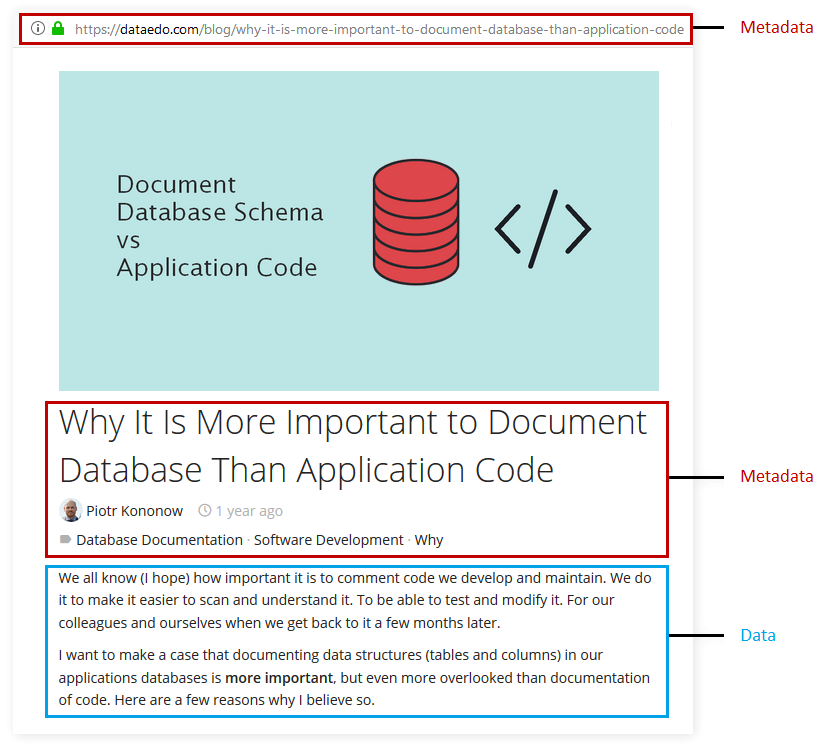
\includegraphics[width=.8\textwidth]{figures/blogmeta}
    \vspace{-5mm}
    \toRight{https://dataedo.com/kb/data-glossary/what-is-metadata}
\end{frame}
\begin{frame}{Emails}
    \centering
    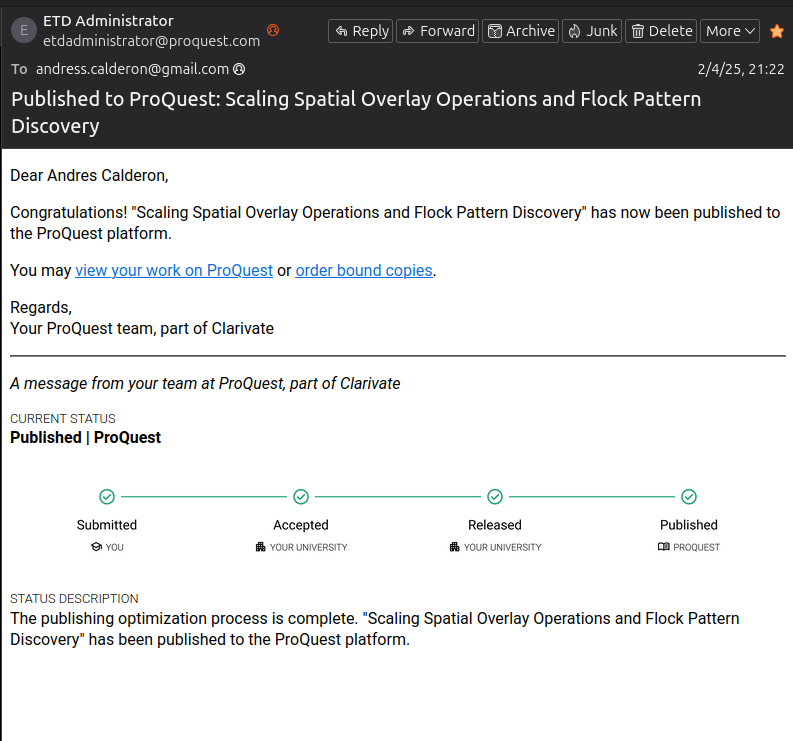
\includegraphics[width=0.75\textwidth]{figures/email}
\end{frame}
\begin{frame}{Email Metadata}
    \centering
    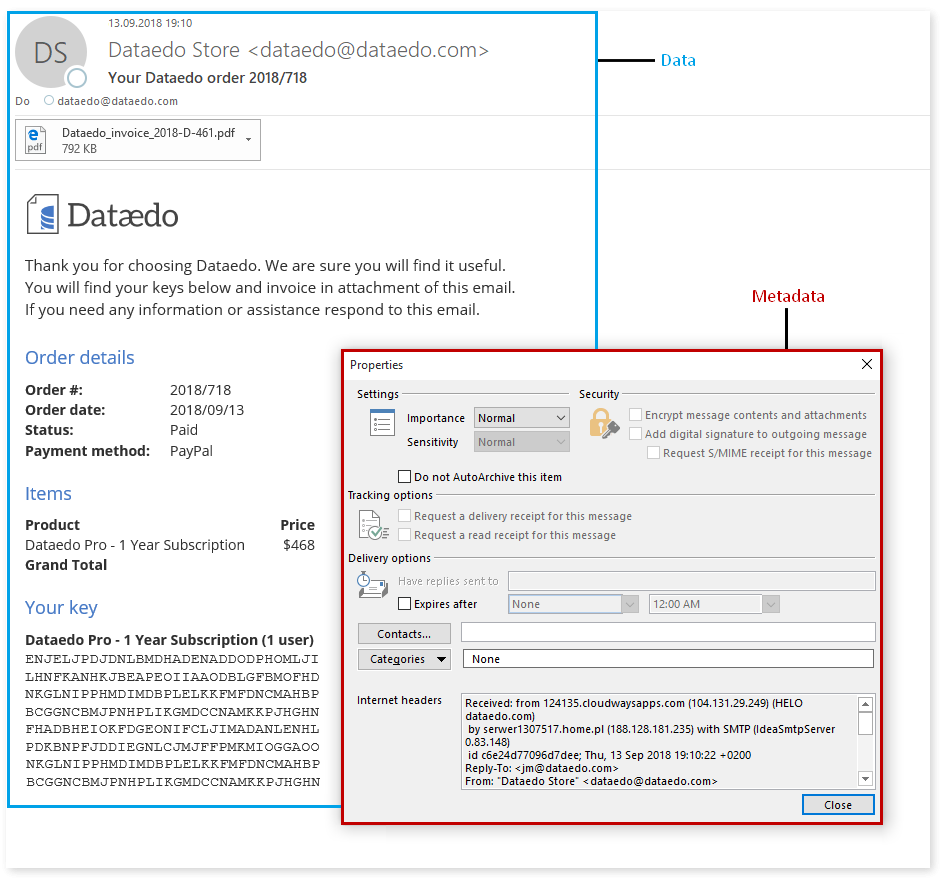
\includegraphics[width=0.75\textwidth]{figures/emailmeta}
\end{frame}
\begin{frame}{Documents}
    \centering
    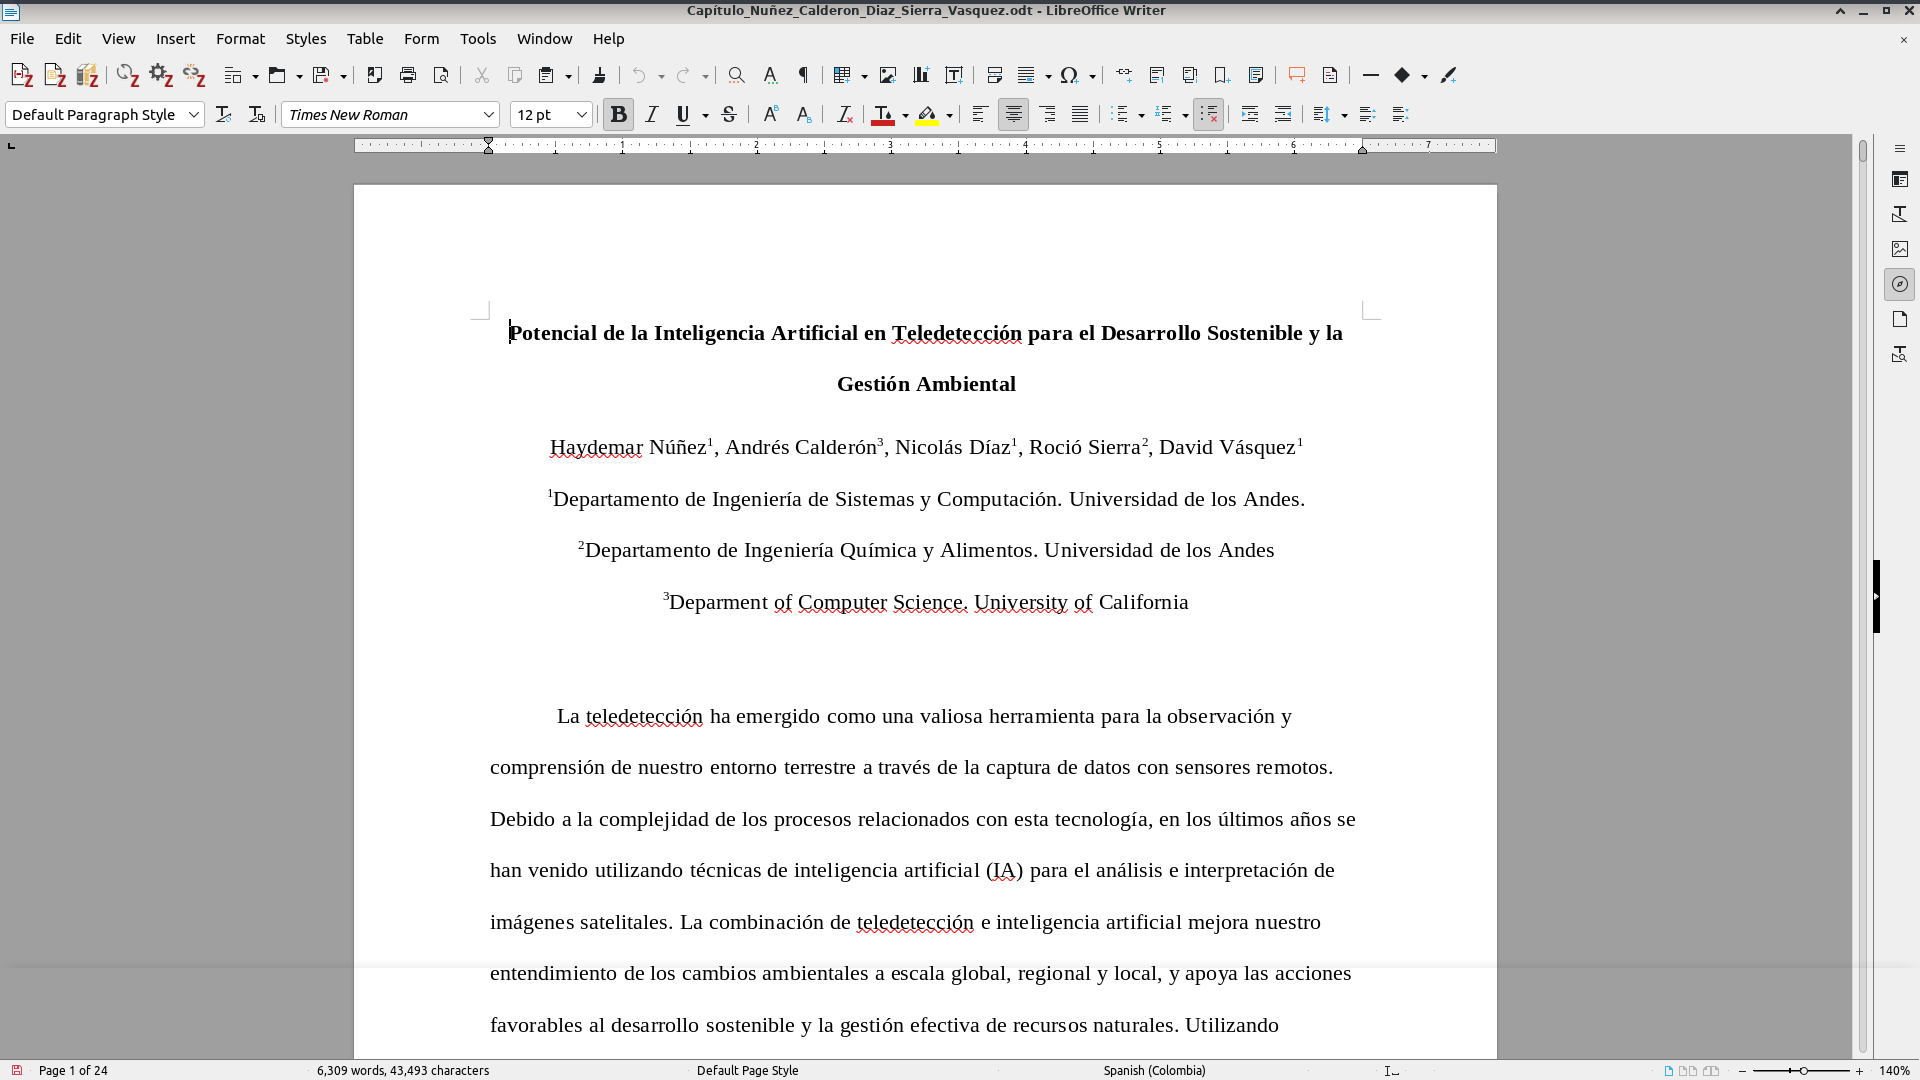
\includegraphics[width=\textwidth]{figures/document}
\end{frame}
\begin{frame}{Document Metadata}
    \centering
    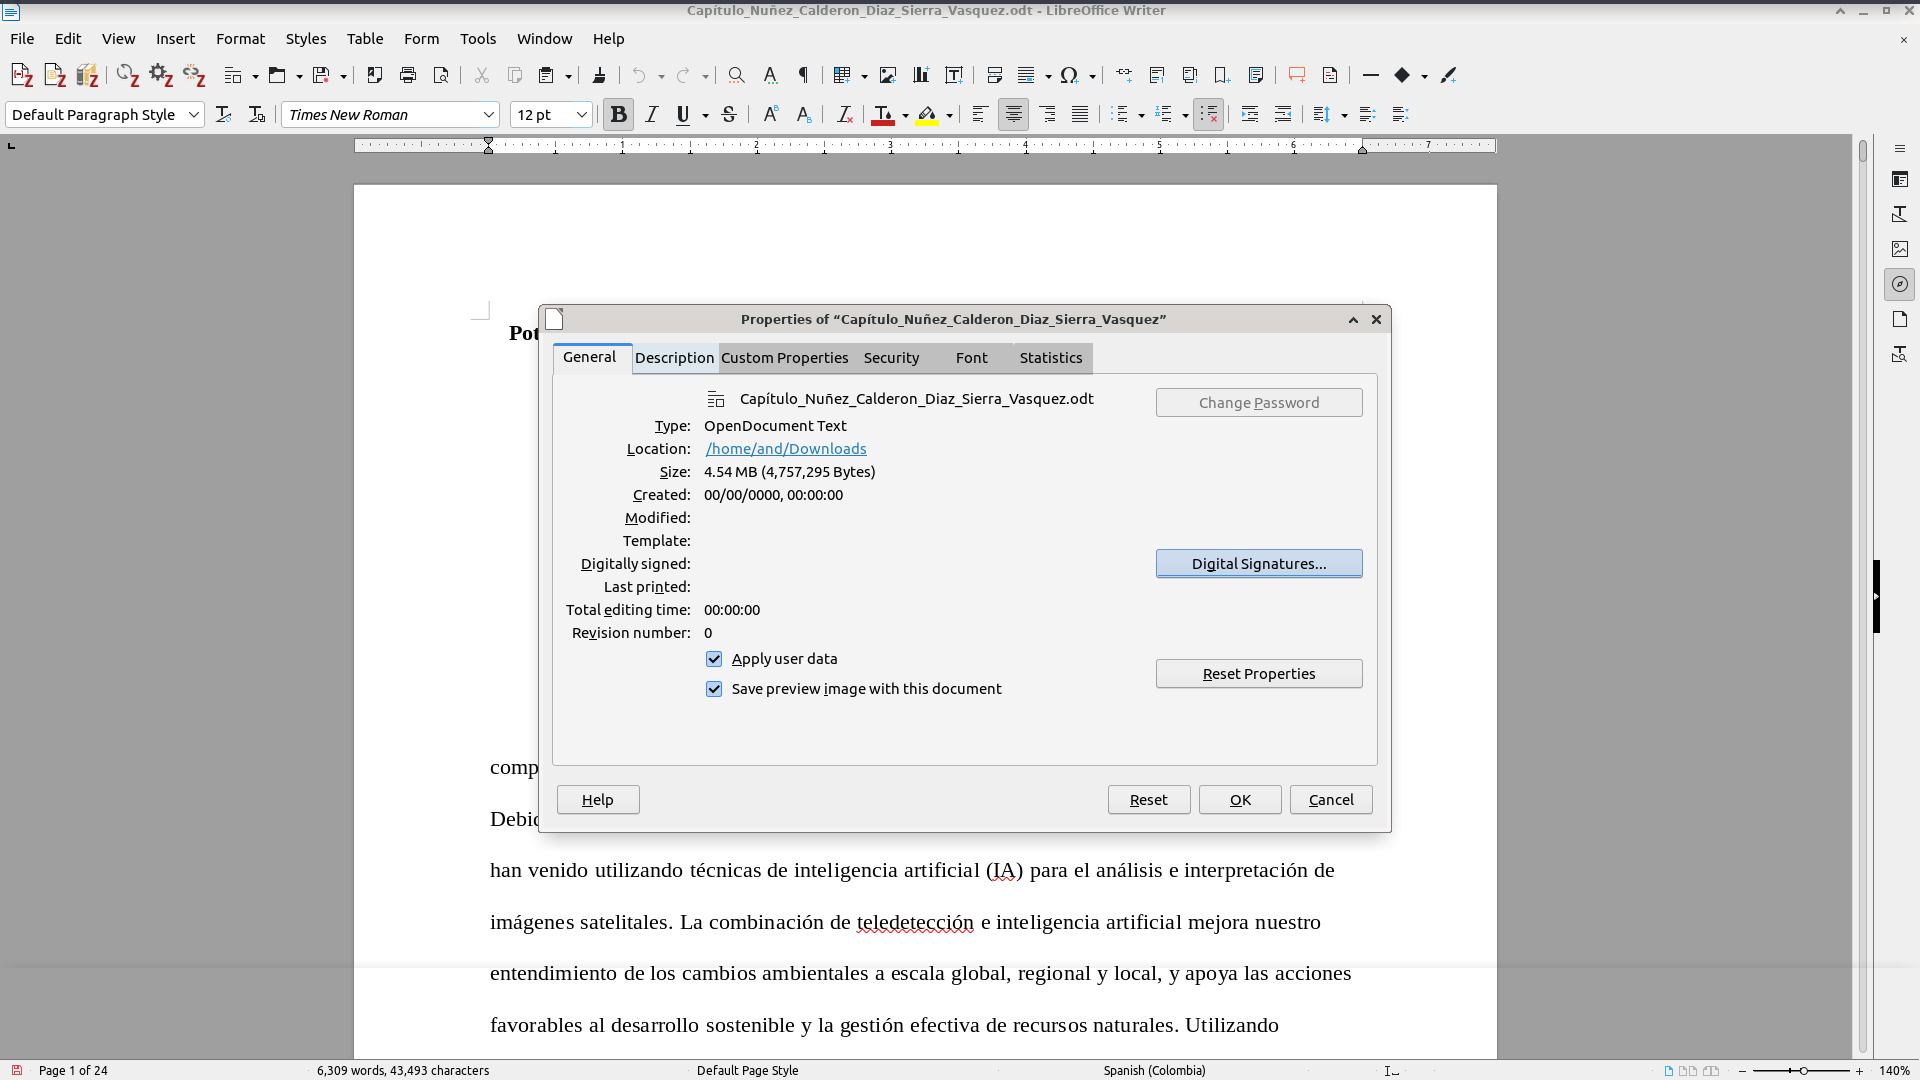
\includegraphics[width=\textwidth]{figures/documentmeta}
\end{frame}
\begin{frame}{Spreadsheets}
    \centering
    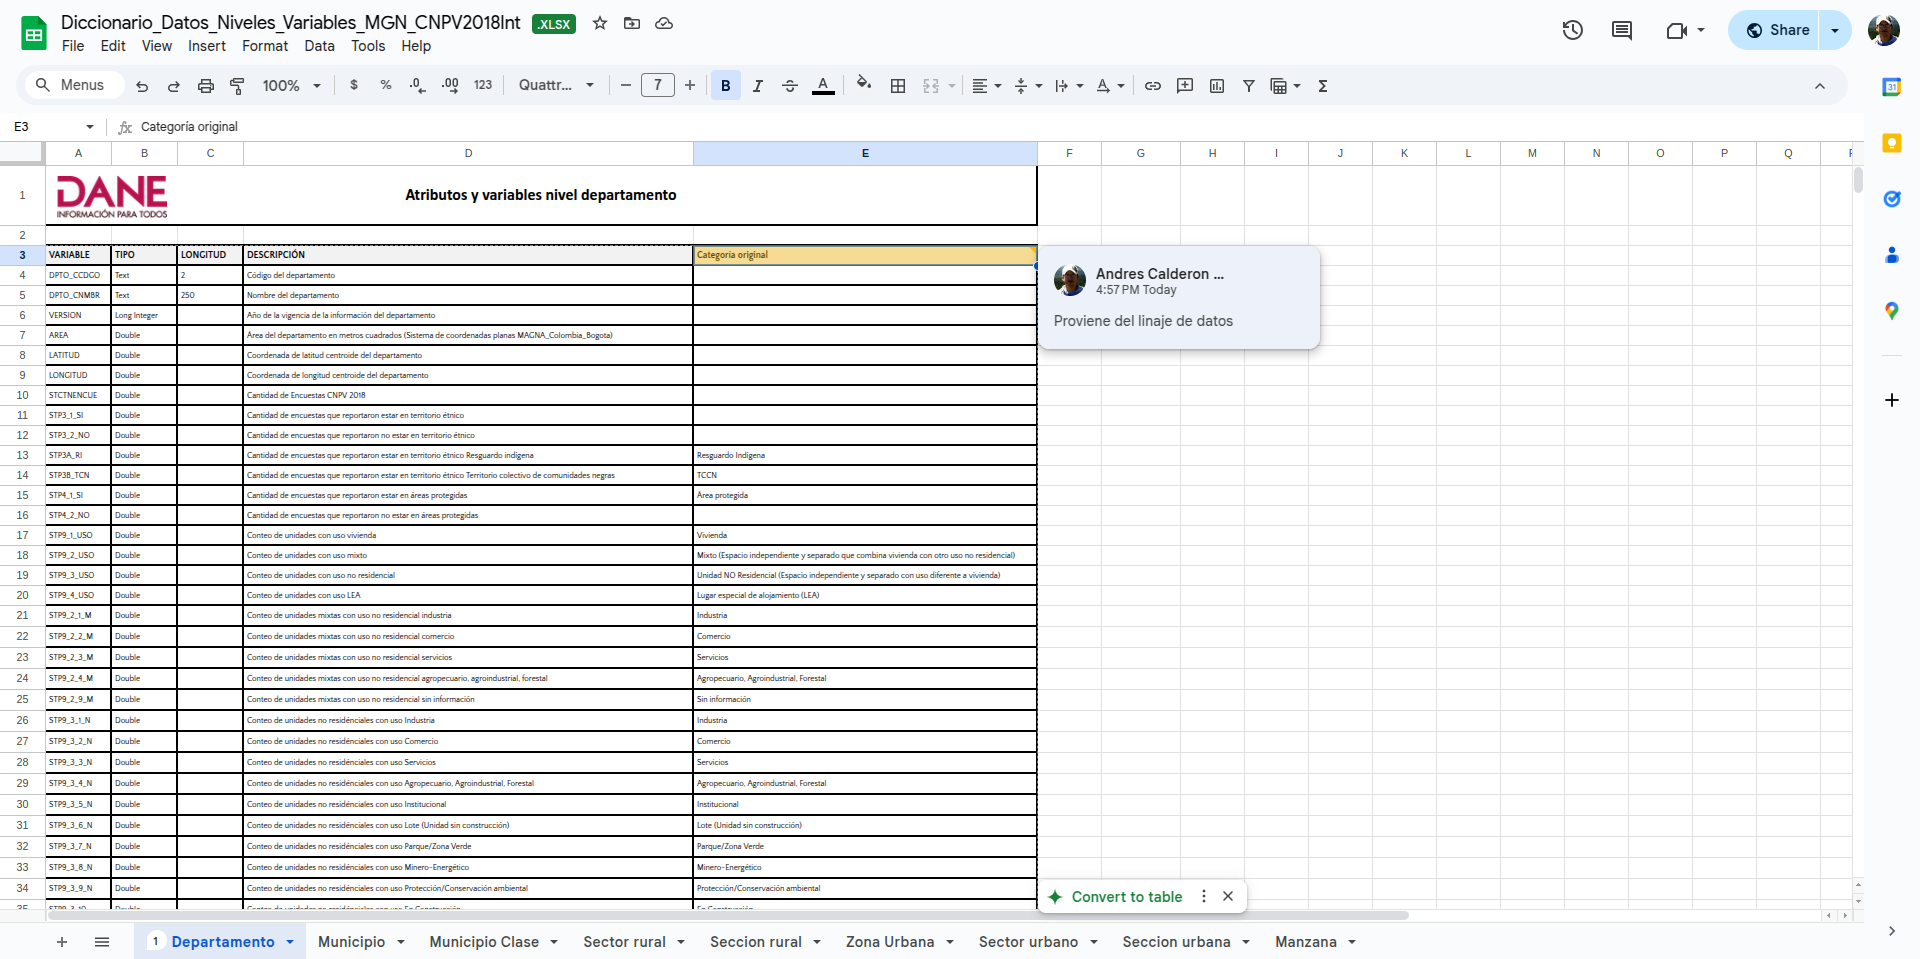
\includegraphics[width=\textwidth]{figures/spreadsheet}
\end{frame}
\begin{frame}{Spreadsheets Metadata}
    \centering
    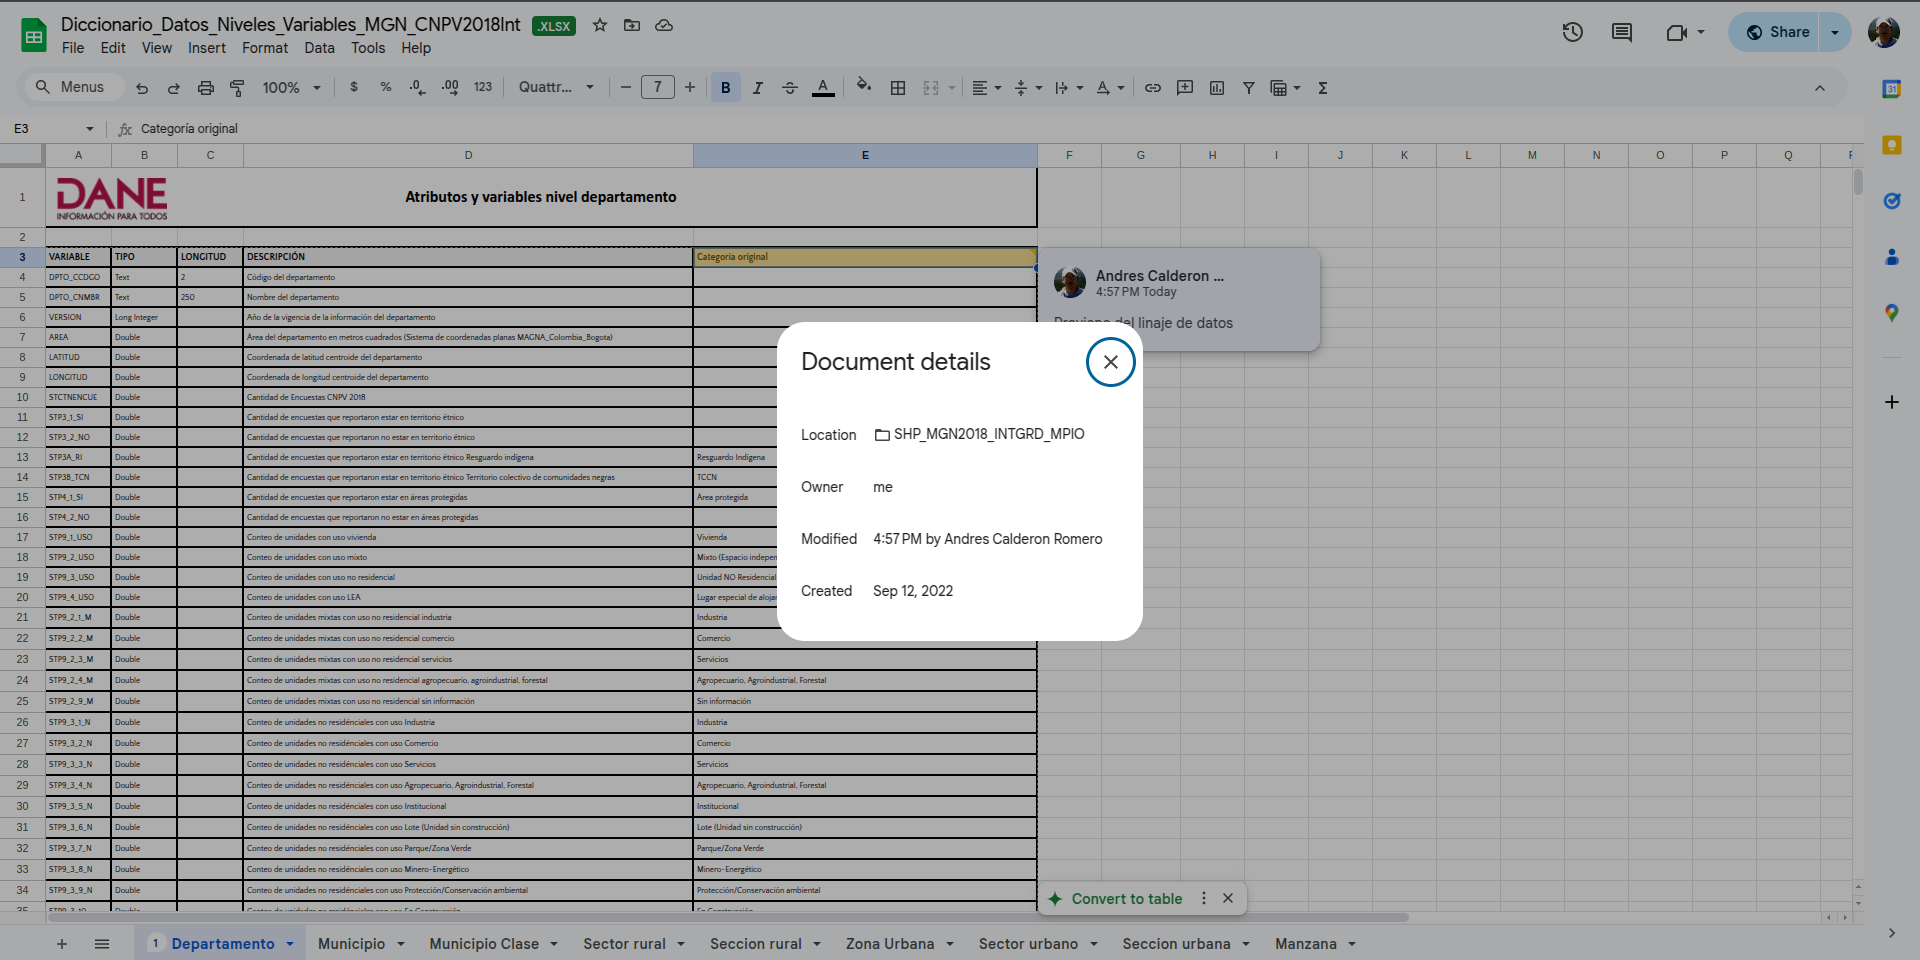
\includegraphics[width=\textwidth]{figures/spreadsheetmeta}
\end{frame}
\begin{frame}{Code}
    \centering
    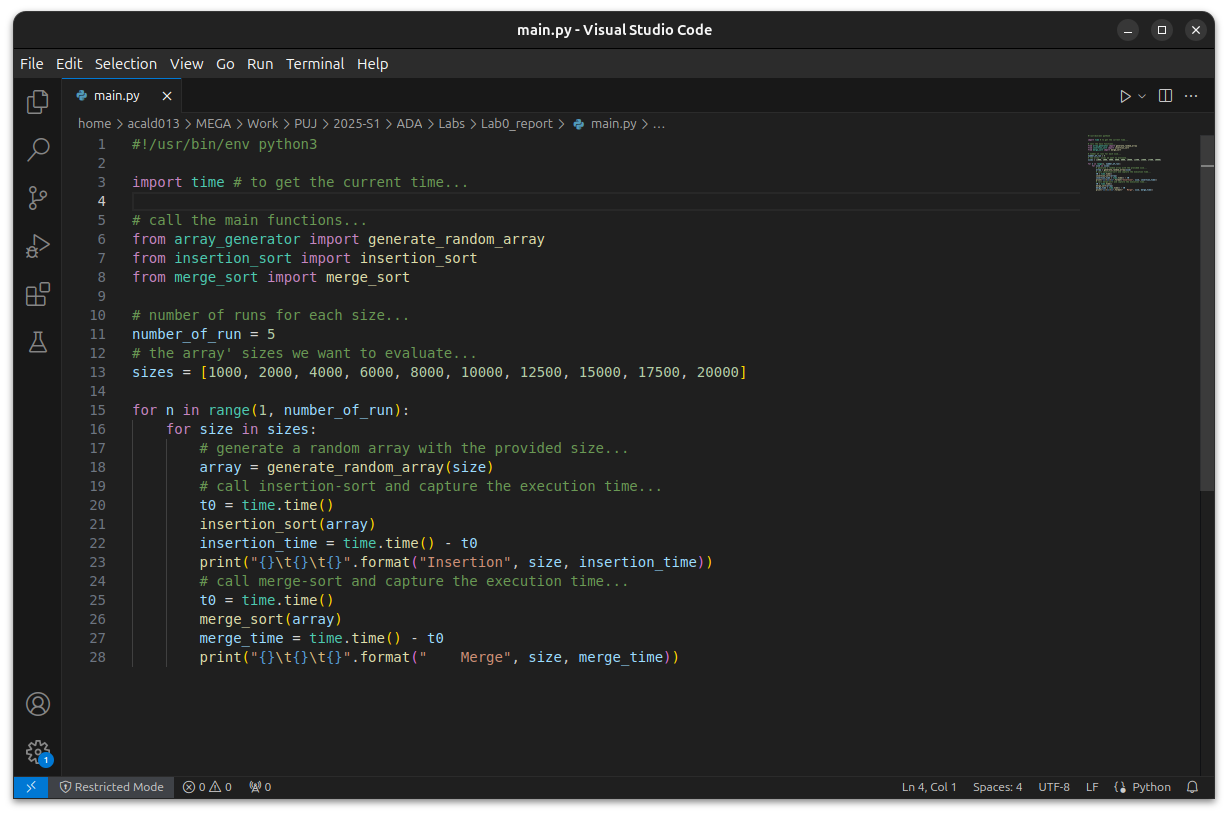
\includegraphics[width=\textwidth]{figures/code}
\end{frame}
\begin{frame}{Code Metadata}
    \centering
    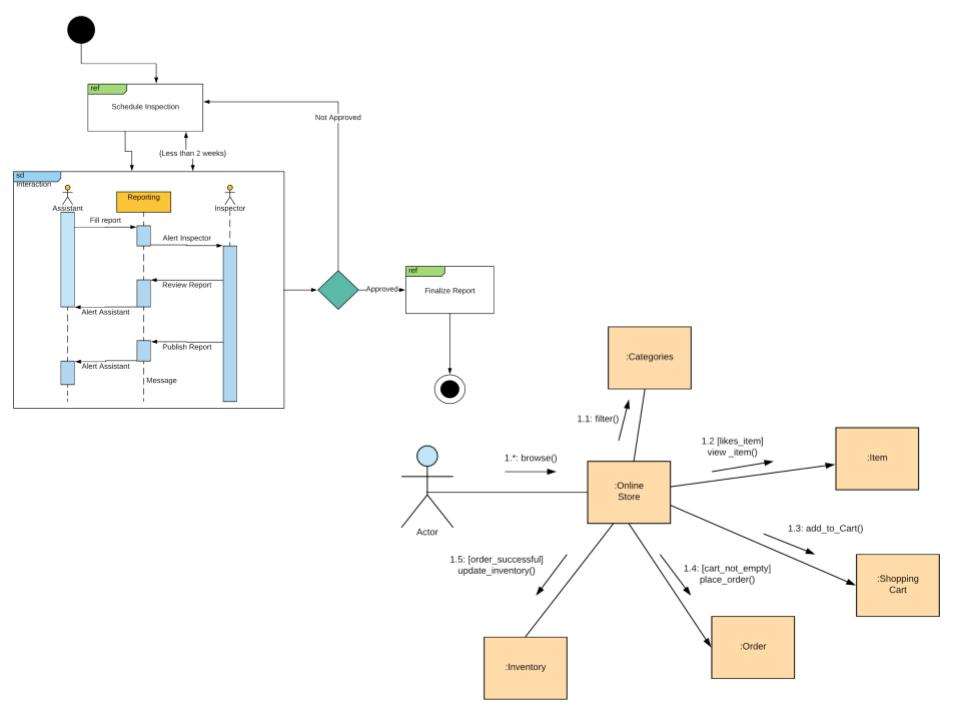
\includegraphics[width=\textwidth]{figures/codemeta}
\end{frame}

\begin{frame}{Databases}
    \centering
    \begin{tikzpicture}[remember picture]
        \path (0,0) node {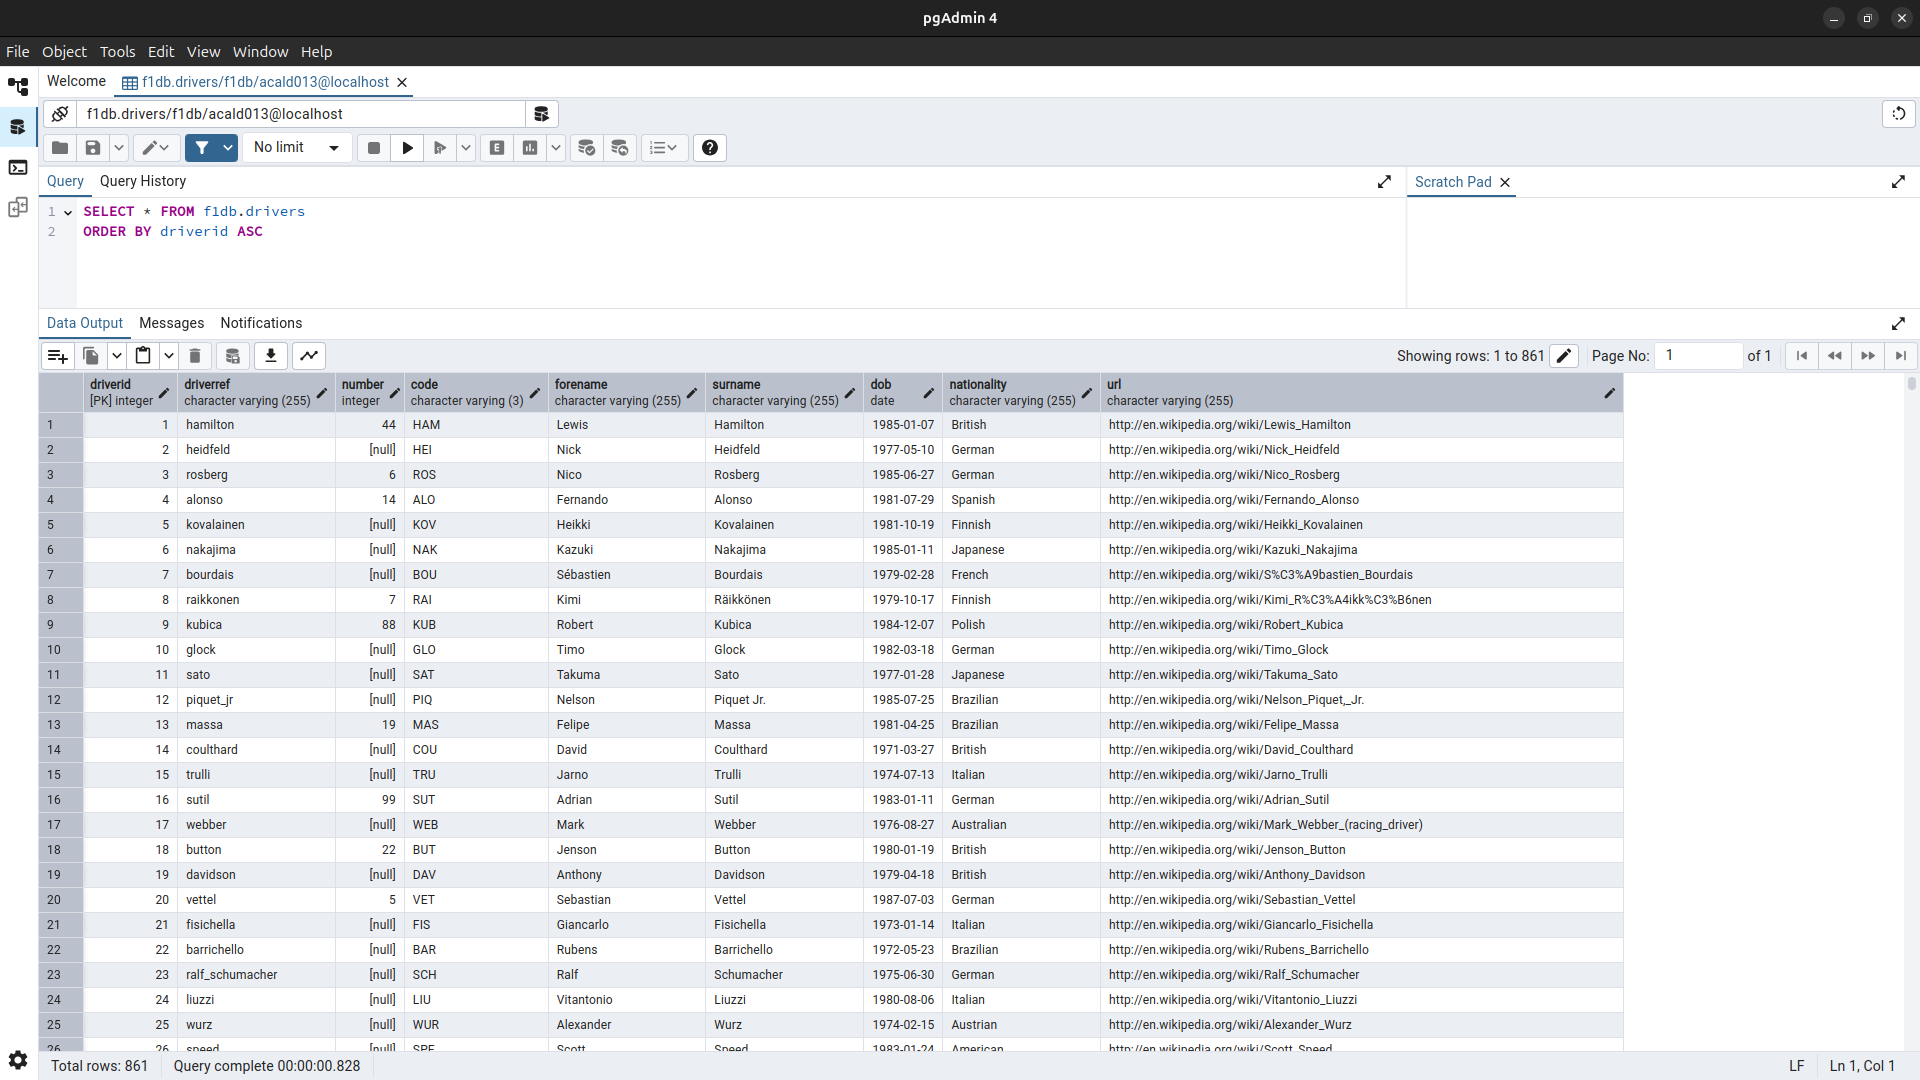
\includegraphics[width=\textwidth]{figures/db}};\pause
        \path (0,0) node {
\includegraphics[width=0.4\textwidth]{figures/qm}};\pause
        \path (0,0) node {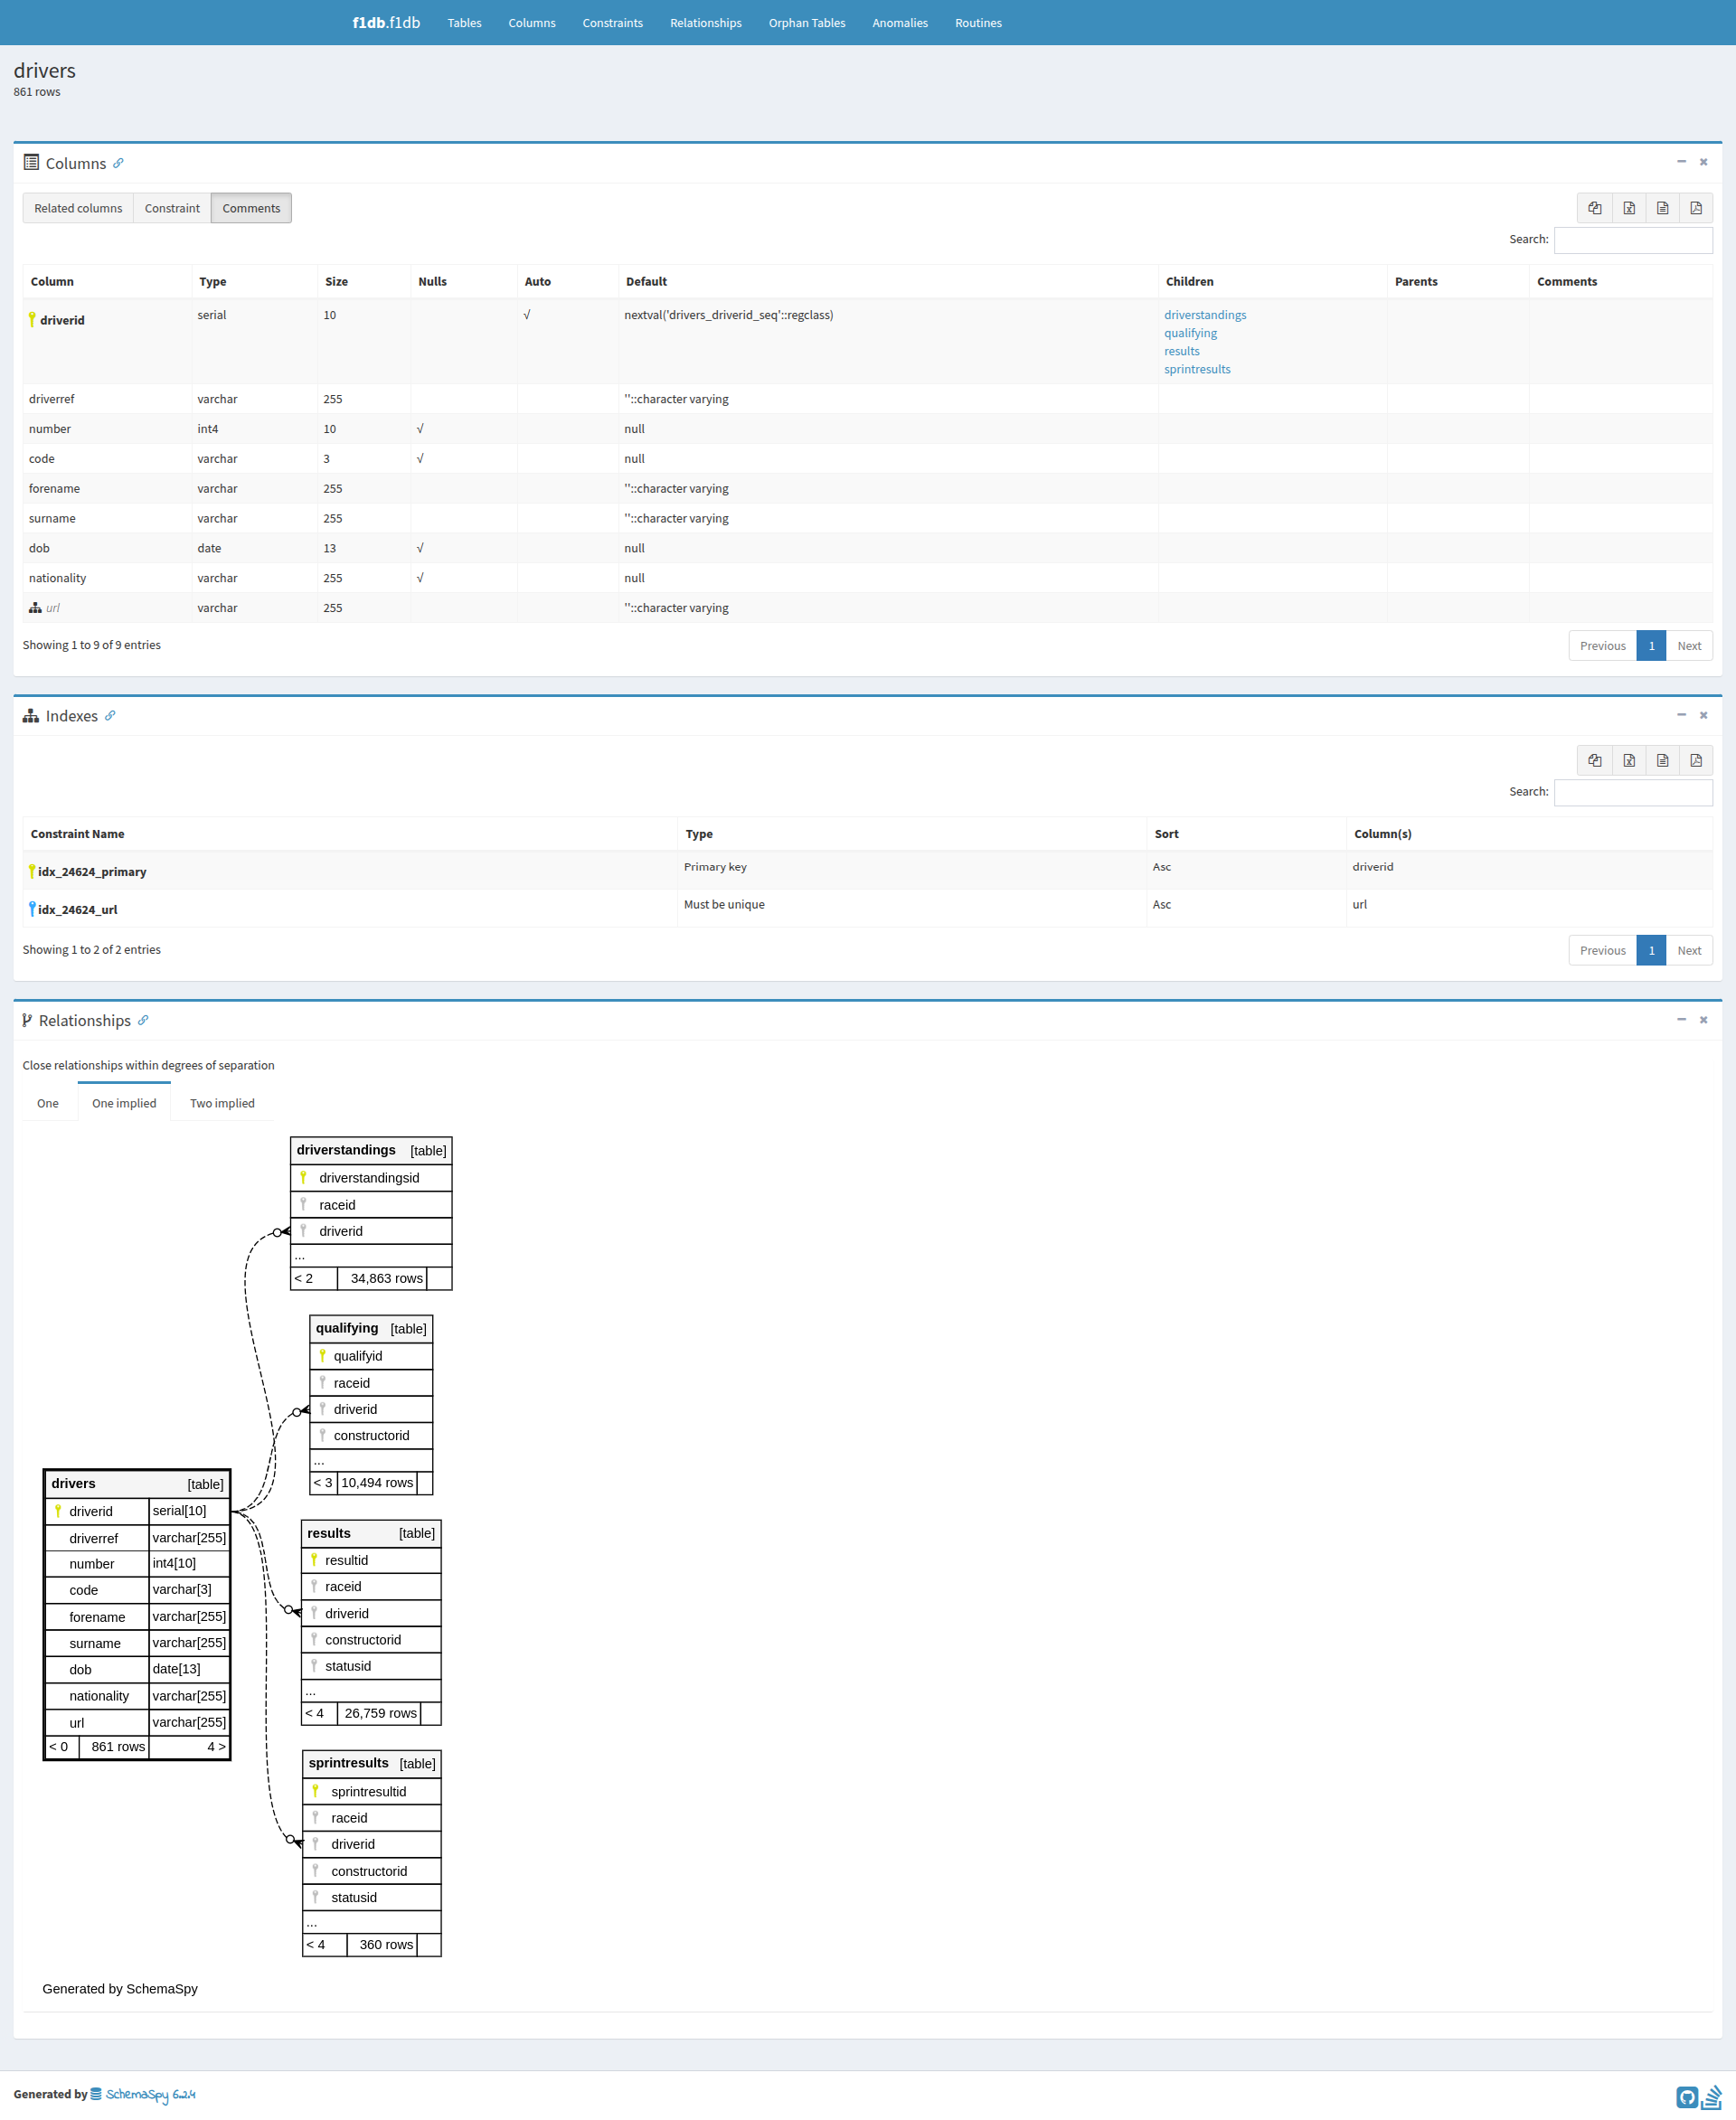
\includegraphics[width=0.625\textwidth]{figures/dbmeta}};
    \end{tikzpicture}
\end{frame}

\begin{frame}{Metadata Characteristics\footnote{Australian Research Data Commons}}
    \footnotesize
    \begin{minipage}{.49\textwidth}
        \begin{itemize}
            \item Metadata is information about an \textit{object} or \textit{resource} that describes \textit{characteristics} of that object, such as content, quality, format, location, and access rights.\pause
            \item Metadata can be used to describe \textit{physical} objects (e.g. samples and specimens) as well as \textit{digital} objects (e.g. documents, images, datasets and software).\pause
            \item Metadata can take many \textit{different forms}, from free text (e.g. a read-me file) to standardised, structured, machine-readable, extensible content.\pause
        \end{itemize}
    \end{minipage}
    \begin{minipage}{.49\textwidth}
        \begin{itemize}
            \item Metadata is \textit{analogous to any other form of data}, in terms of how it is created, managed, linked and stored.\pause
            \item Metadata is \textit{associated with} the data it describes.  It can be embedded within the data file, or recorded a separated text/spreadsheet file that is linked to the collection of data files it describes, or contained in a catalogue record that points to the research data collection.\pause
            \item Metadata \textit{enables} and \textit{enhances} the \textit{discovery} and \textit{reuse} of data.\pause
        \end{itemize}
    \end{minipage}
\end{frame}

\section{Database Administration Tools}

\begin{frame}
    \frametitle{DBA Tools}
    The Data Dictionary (aka Metadata repository)
    \begin{itemize}
        \item Is a database administartion tool.
        \item It is a type of metada itself.
        \item Oracle defines it as a collection of tables with metadata.
    \end{itemize}

    \begin{alertblock}{Definition}
        A data dictionary is a ``\textit{centralized repository of information about data such as meaning, relationships to other data, origin, usage, and format.}''
    \end{alertblock}
\end{frame}

\begin{frame}{Data Dictionary}
    \small
    \begin{minipage}{.40\textwidth}
        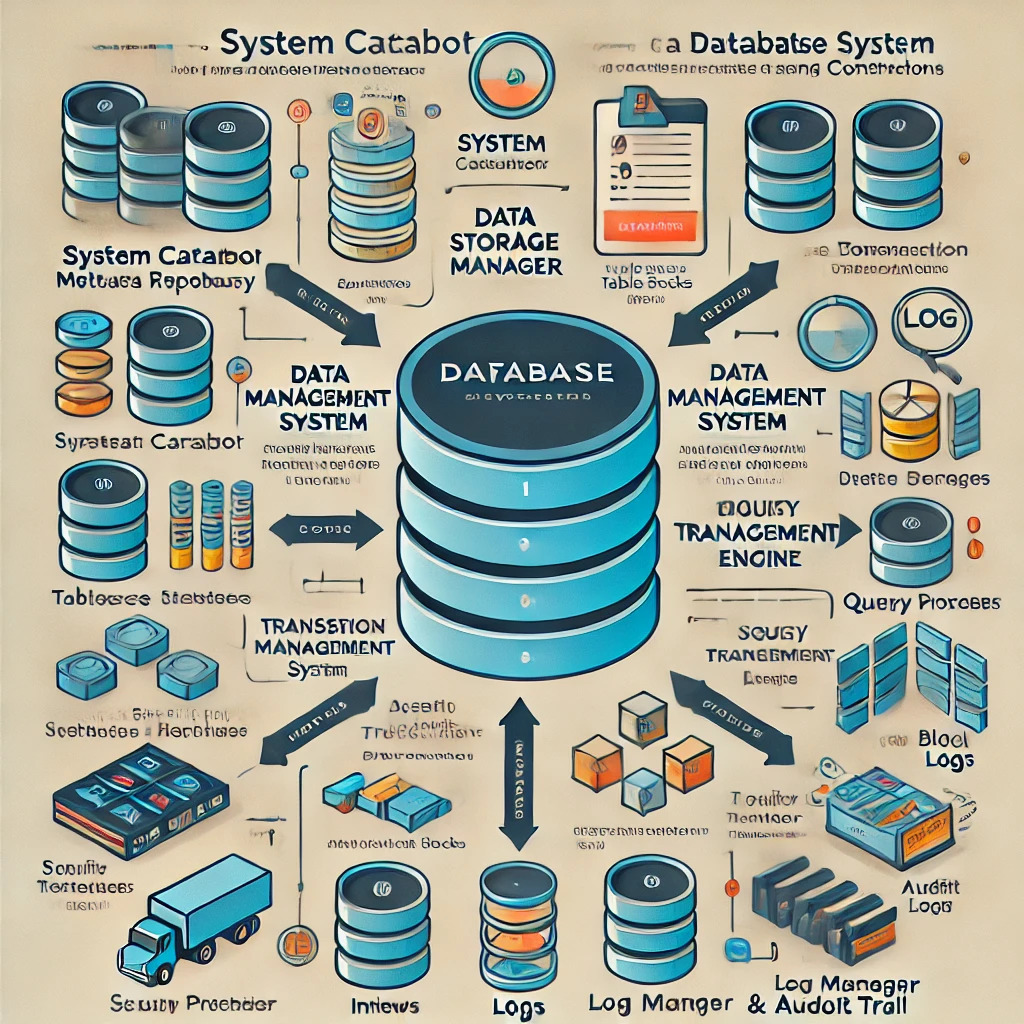
\includegraphics[width=\textwidth]{figures/dd}
    \end{minipage}\hfill
    \begin{minipage}{.55\textwidth}
        \tiny
        DD stores information about database objects, including:
        \begin{itemize}
            \item Tables (names, columns, data types, constraints). \pause
            \item Indexes (primary keys, foreign keys). \pause
            \item Views (virtual tables). \pause
            \item Users \& Permissions (who can access what). \pause
            \item Storage Structures (tablespaces, partitions). \pause
            \item Relationships \& Dependencies (links between tables). \pause
            \item Audit \& Logs (history of schema changes).
        \end{itemize}
    \end{minipage}
\end{frame}

\begin{frame}
    \frametitle{Data Dictionary Types}
    \begin{itemize}
        \item \textbf{Integrated:}
            \begin{itemize}
                \item With the DBMS. i.e., relational DBMSs include a built-in DD or system catalog that is frequently accessed and updated by the RDBMS.
                \item Tend to limit their metadata to the data managed by the DBMS.
            \end{itemize} \pause

        \item \textbf{Standalone:}
            \begin{itemize}
                \item Other DBMSs, especially older types, do not have a built-in data dictionary; instead, the DBA may use third-party standalone systems.
                \item Usually more flexible and allow the DBA to describe and manage all of the organization's data, whether they are computerized or not.
            \end{itemize}
    \end{itemize}
\end{frame}

\begin{frame}
    \frametitle{Data Dictionary Types}
    \begin{itemize}
        \item \textbf{Active:} Automatically updated by the DBMS with every database access to keep its access information up to date. \pause
        \item \textbf{Passive:} Not updated automatically and usually DBA requires running a batch process.
    \end{itemize}
\end{frame}

\begin{frame}
    \frametitle{Data Dictionary Function}
    \begin{itemize}
        \item The DD main function is to store the description of all objects that interact with the database.
        \item Whatever the data dictionary’s format, it provides database designers and end users with a much-improved ability to communicate.
        \item The DD is the tool that helps the DBA resolve data conflicts.
    \end{itemize}
\end{frame}

\begin{frame}
    \frametitle{Data Dictionary Content\footnote{More info in \textit{``Database Systems: Design, Implementation, \& Management.''} $13^{th} Ed.$ (Coronel \& Morris, 2017). Section 16-7a.}}
    Although there is no standard format for the information stored in the DD, several features are common. DD typically stores descriptions of the following:
    \begin{itemize}
        \item Data elements that are defined in all tables of all databases.\pause
        \item Tables defined in all databases.\pause
        \item Indexes defined for each database table.\pause
        \item Defined databases.\pause
        \item End users and administrators of the database.\pause
        \item Programs that access the database.\pause
        \item Access authorizations for all users of all databases.\pause
        \item Relationships among data elements.\pause
    \end{itemize}
\end{frame}


\section{Understanding PostgreSQL System Catalogs}

\begin{frame}
    \frametitle{What are PostgreSQL System Catalogs?}
    \begin{itemize}
        \item Internal tables where PostgreSQL stores schema metadata.
        \item Contain information about databases, tables, columns, and more.
        \item Essential for managing and querying database structure.
    \end{itemize}
\end{frame}

\begin{frame}
    \frametitle{Naming Conventions}
    \begin{itemize}
        \item Catalog names start with \texttt{pg\_}.
        \item Column prefixes often derived from catalog names:
        \begin{itemize}
            \item \texttt{pg\_database}: columns start with \texttt{dat\_} (e.g., \texttt{datname}).
            \item \texttt{pg\_proc}: columns start with \texttt{pro\_}.
            \item \texttt{pg\_namespace}: columns start with \texttt{nsp\_}.
            \item \texttt{pg\_class}: columns start with \texttt{rel\_} (stores information about tables and other objects with columns, referred to as ``relations'').
        \end{itemize}
    \end{itemize}
\end{frame}

\begin{frame}[fragile]
    \frametitle{Retrieving Database Metadata}
    \begin{itemize}
        \item \texttt{pg\_database} stores information about databases.
        \item To find the owner of a specific database:
    \end{itemize}
    \begin{minted}
    [tabsize=4, obeytabs, frame=lines, framesep=2mm, baselinestretch=1.2, bgcolor=LightGray, fontsize=\scriptsize, linenos]{sql}
    SELECT
        a.rolname AS 'Owner'
    FROM
        pg_database d
    JOIN
        pg_authid a
    ON
        a.oid = d.datdba
    WHERE
        datname = 'your_database_name';
    \end{minted}
    \begin{itemize}
        \item Replace \texttt{your\_database\_name} with the name of your database.
    \end{itemize}
\end{frame}

\begin{frame}[fragile]
    \frametitle{Retrieving Table Metadata}
    \begin{itemize}
        \item \texttt{pg\_class} stores information about tables, indexes, and views.
        \item To list all ordinary tables:
    \end{itemize}
    \begin{minted}
    [tabsize=4, obeytabs, frame=lines, framesep=2mm, baselinestretch=1.2, bgcolor=LightGray, fontsize=\scriptsize]{sql}
    SELECT
        relname
    FROM
        pg_class
    WHERE
        relkind = 'r';
    \end{minted}
    \begin{itemize}
        \item \texttt{relkind = `r'} indicates ordinary tables.
    \end{itemize}
\end{frame}

\begin{frame}[fragile]
    \frametitle{Retrieving Schema Metadata}
    \begin{itemize}
        \item \texttt{pg\_namespace} stores information about schemas.
        \item To list all schema names:
    \end{itemize}
    \begin{minted}
    [tabsize=4, obeytabs, frame=lines, framesep=2mm, baselinestretch=1.2, bgcolor=LightGray, fontsize=\scriptsize]{sql}
    SELECT
        nspname
    FROM
        pg_namespace;
    \end{minted}
\end{frame}

\begin{frame}[fragile]
    \frametitle{Retrieving Index Metadata}
    \begin{itemize}
        \item \texttt{pg\_index} and \texttt{pg\_class} store information about indexes.
        \item To find tables without indexes:
    \end{itemize}
    \begin{minted}
    [tabsize=4, obeytabs, frame=lines, framesep=2mm, baselinestretch=1.2, bgcolor=LightGray, fontsize=\scriptsize, linenos]{sql}
    SELECT
        c.oid::regclass AS table_name
    FROM
        pg_class c
    WHERE
        relkind = 'r' AND NOT EXISTS (
            SELECT 1 FROM pg_index i WHERE i.indrelid = c.oid
        );
    \end{minted}
\end{frame}

\begin{frame}[fragile]
    \frametitle{Retrieving Column Metadata}
    \begin{itemize}
        \item \texttt{pg\_attribute} stores information about table columns.
        \item To list column names and their data types:
    \end{itemize}
    \begin{minted}
    [tabsize=4, obeytabs, frame=lines, framesep=2mm, baselinestretch=1.2, bgcolor=LightGray, fontsize=\scriptsize, linenos]{sql}
    SELECT
        attname, atttypid::regtype
    FROM
        pg_attribute LIMIT 50;
    \end{minted}
    \begin{itemize}
        \item The \texttt{regtype} cast provides human-readable data types.
    \end{itemize}
\end{frame}

\begin{frame}[fragile]
    \frametitle{Retrieving Function Metadata}
    \begin{itemize}
        \item \texttt{pg\_proc} stores information about functions.
        \item To find functions that accept a \texttt{text} argument:
    \end{itemize}
    \begin{minted}
    [tabsize=4, obeytabs, frame=lines, framesep=2mm, baselinestretch=1.2, bgcolor=LightGray, fontsize=\scriptsize, linenos]{sql}
    SELECT
        oid::regprocedure
    FROM
        pg_proc
    WHERE
        'text'::regtype = ANY(proargtypes);
    \end{minted}
\end{frame}

\begin{frame}[fragile]
    \frametitle{Retrieving Size Information}
    \begin{itemize}
        \item To get the size of tables:
    \end{itemize}
    \begin{minted}
    [tabsize=4, obeytabs, frame=lines, framesep=2mm, baselinestretch=1.2, bgcolor=LightGray, fontsize=\scriptsize, linenos]{sql}
    SELECT
        oid::regclass AS table_name,
        pg_size_pretty(pg_table_size(oid)) AS size
    FROM
        pg_class
    WHERE
        relkind = 'r'
    ORDER BY
        pg_table_size(oid) DESC;
    \end{minted}
    \begin{itemize}
        \item \texttt{pg\_size\_pretty} formats sizes into readable units.
    \end{itemize}
\end{frame}

\begin{frame}{}
    \centering
    \Huge End of Lecture 3.
\end{frame}

\section*{Takeaways}

% Tim Duncan's Top 5 Fundamental Takeaways of the Today's Class
\begin{frame}{TDT5FTOTTC}
    \centering
    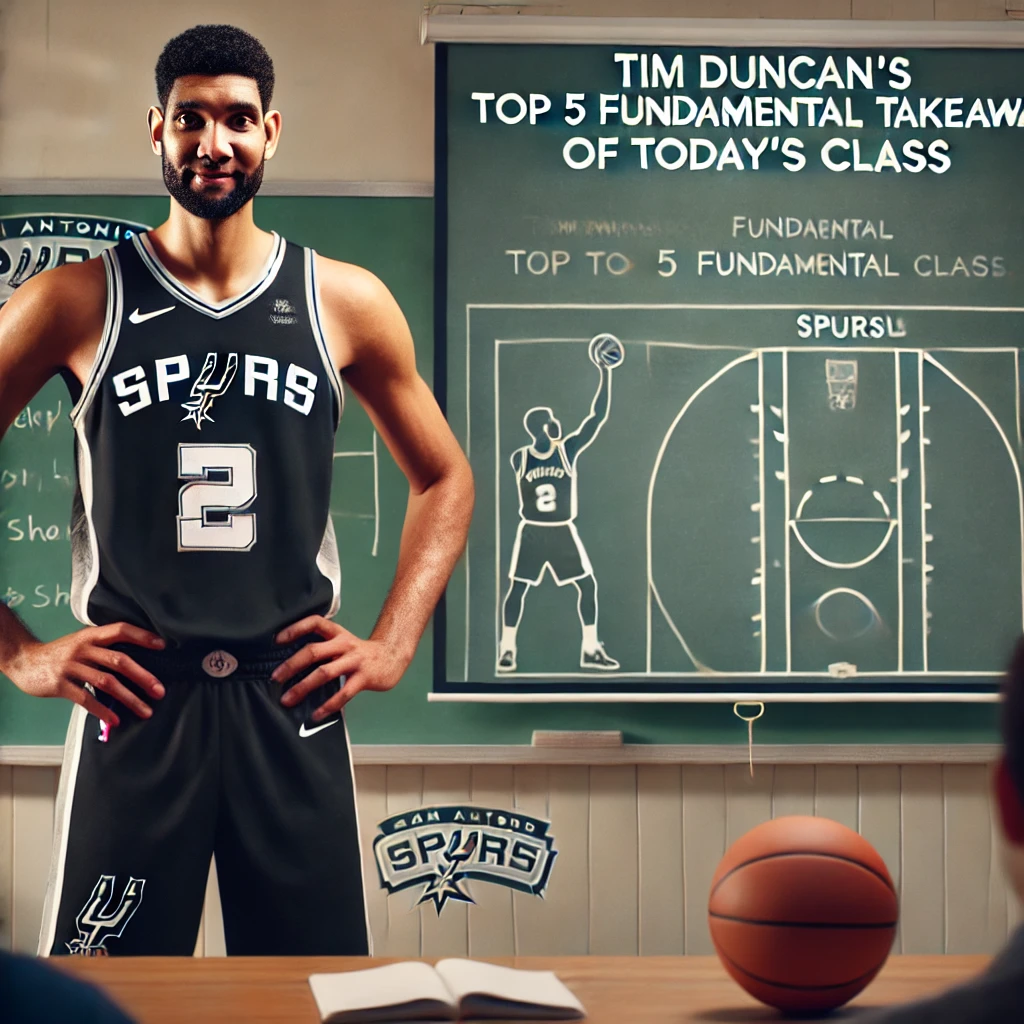
\includegraphics[width=0.75\textwidth]{figures/tim.png}
\end{frame}

\begin{frame}{Top 5 Fundamental Takeaways}
    \begin{enumerate} \pause
        \item[5] \textbf{PostgreSQL uses system catalogs} to store metadata about databases, tables, schemas, and indexes, helping administrators manage the database.\pause
        \item[4] \textbf{SQL queries can retrieve metadata} to list tables, schemas, indexes, and data sizes, making database management more efficient.\pause
        \item[3] \textbf{Metadata can be structured or unstructured} and is used to describe both digital and physical objects for better data discovery and reuse.\pause
        \item[2] \textbf{Metadata is data about data}, describing properties like type, size, and relationships to help organize and manage information.\pause
        \item[1] \textbf{The Data Dictionary} is a key tool in database administration, storing details about tables, indexes, users, and permissions.
        \end{enumerate}
\end{frame}

\begin{frame}{Database Administration: What is Metadata?}
    \centering
    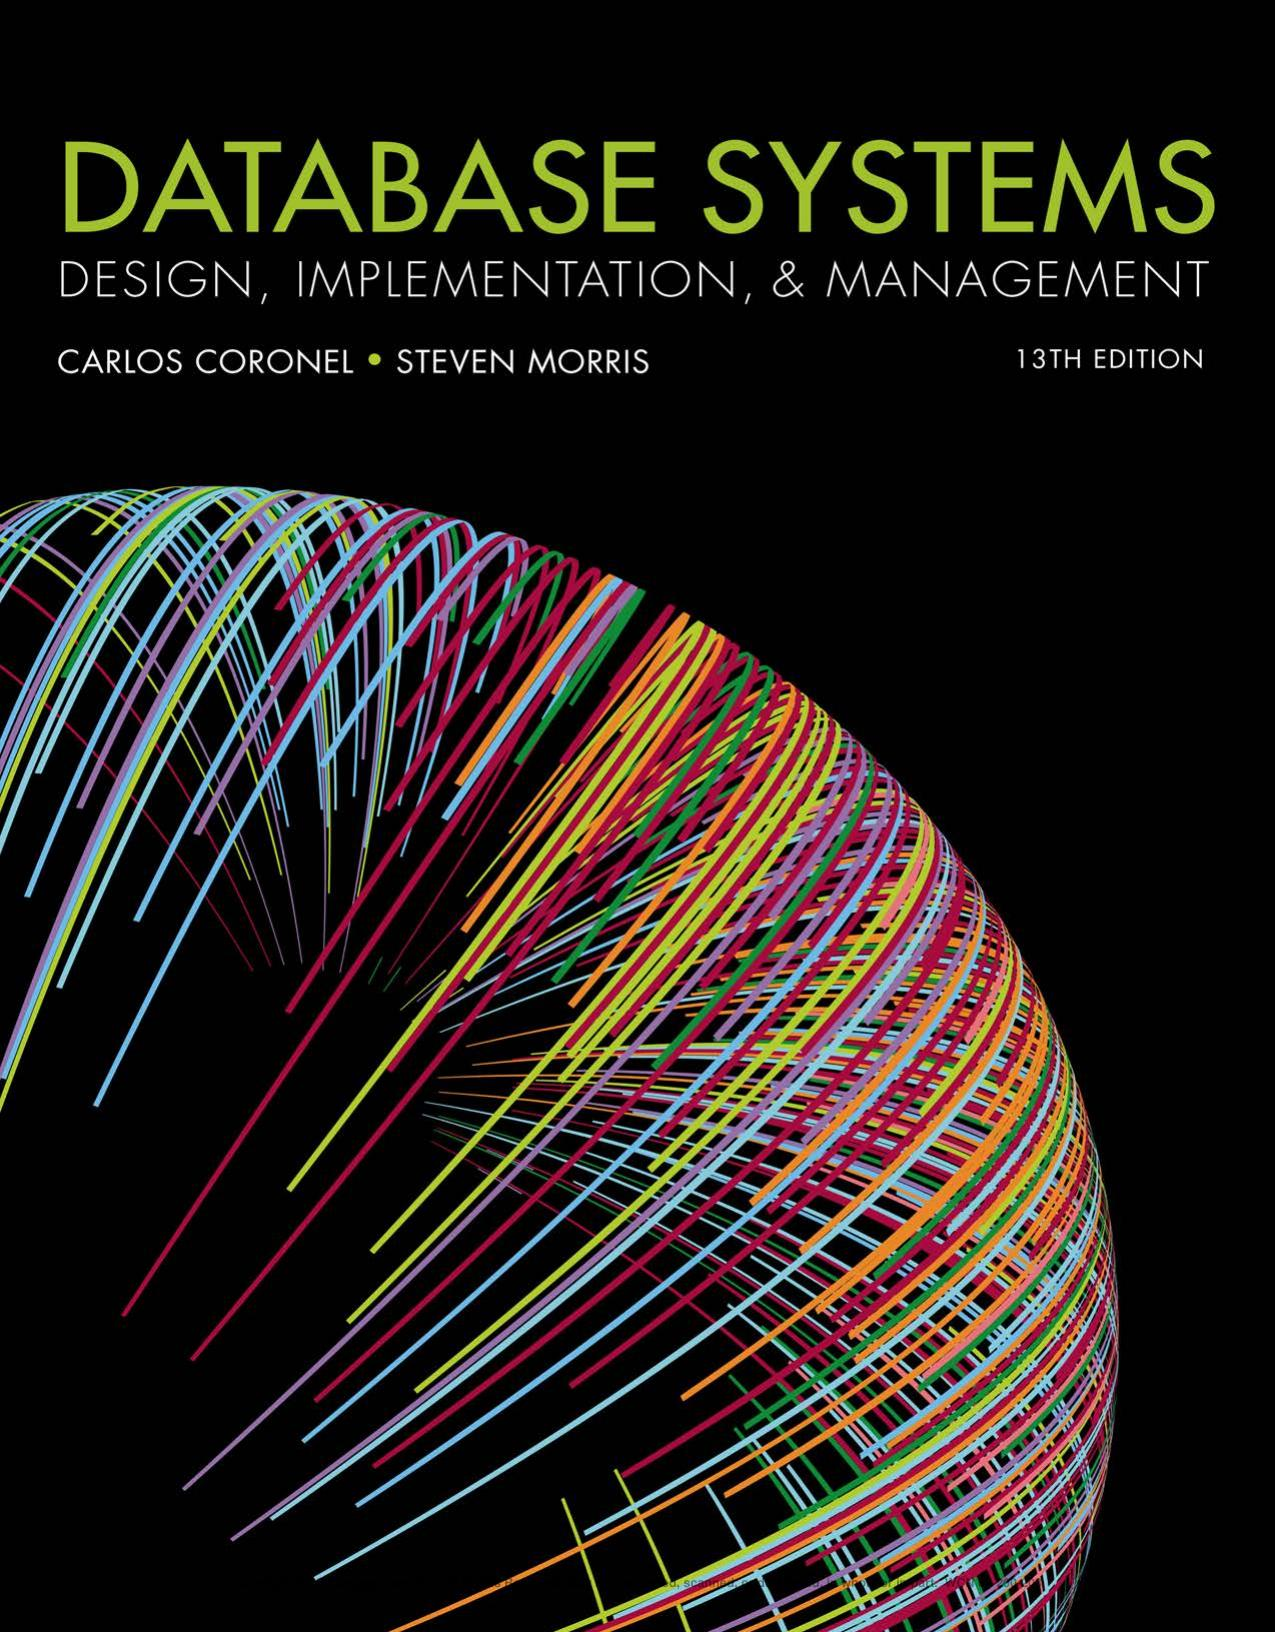
\includegraphics[width=0.34\textwidth]{figures/book_cover2.jpg}
    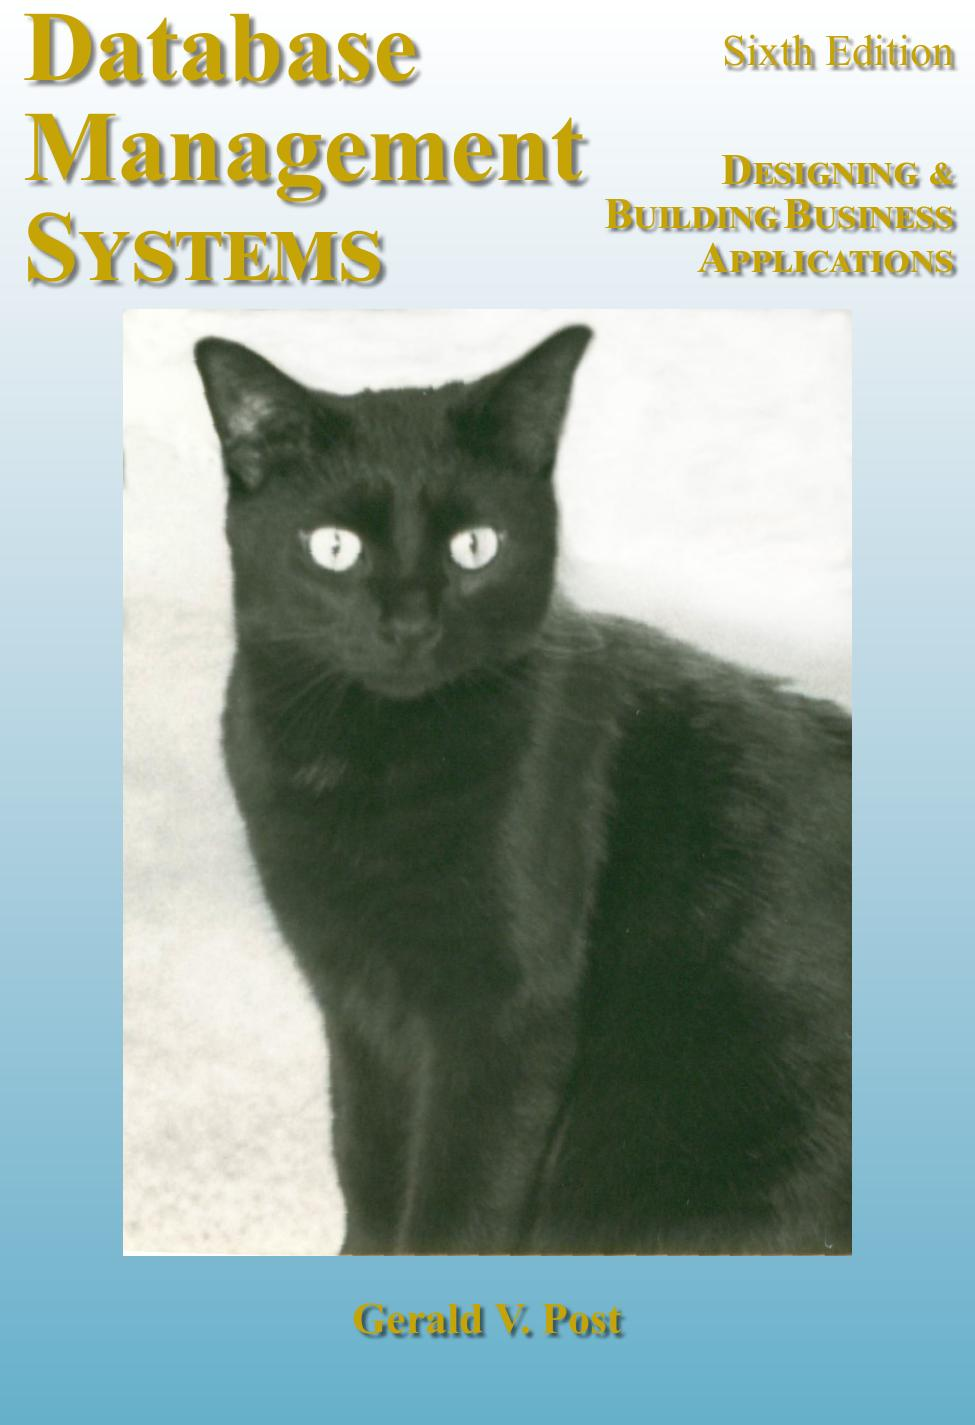
\includegraphics[width=0.3\textwidth]{figures/book_cover3.jpg} \\
    \vspace{5mm}
    {
        \tiny
        Content has been extracted from \textit{Database Systems: Design, Implementation, and Management.}, 13th Edition, by Carlos Coronel \& Steven Morris. Cengage Learning. 2018. and \textit{Database Management Systems: Designing \& Building Business Applications.}, 6th Edition, by Gerald Post. McGraw-Hill/Irwin. 2014. \\
        Visit \url{https://www.cengage.com/c/database-systems-design-implementation-management-13e-coronel/9781337627900PF/} and \url{https://www.jerrypost.com/database/DBBookSummary.html}.\\
    }
\end{frame}

\end{document}
